% !TEX program = xelatex
\documentclass[11pt,a4paper]{article}

\usepackage[top=2.5cm,bottom=2.5cm,left=2.5cm,right=2.5cm]{geometry}
\usepackage{fontspec}
\usepackage{lmodern}
\usepackage{graphicx}
\usepackage{booktabs}
\usepackage{hyperref}
\usepackage{xcolor}
\usepackage{listings}
\usepackage{float}
\usepackage{enumitem}
\usepackage{amsmath}
\usepackage{amssymb}
\usepackage{tabularx}
\usepackage{caption}
\usepackage{subcaption}
\usepackage{longtable}
\usepackage{fancyhdr}
\usepackage{titlesec}

% lmodern provides the fonts; fontspec picks them up automatically with xelatex

\hypersetup{
  colorlinks=true,
  linkcolor=blue!60!black,
  citecolor=green!50!black,
  urlcolor=blue!70!black
}

\definecolor{codebg}{rgb}{0.95,0.95,0.95}
\definecolor{codeframe}{rgb}{0.8,0.8,0.8}

\lstset{
  basicstyle=\small\ttfamily,
  backgroundcolor=\color{codebg},
  frame=single,
  rulecolor=\color{codeframe},
  breaklines=true,
  captionpos=b,
  tabsize=2
}

\titleformat{\section}{\Large\bfseries}{\thesection}{1em}{}
\titleformat{\subsection}{\large\bfseries}{\thesubsection}{1em}{}
\titleformat{\subsubsection}{\normalsize\bfseries}{\thesubsubsection}{1em}{}

\pagestyle{fancy}
\fancyhf{}
\fancyhead[L]{\small\leftmark}
\fancyhead[R]{\small SSLE -- Project 1}
\fancyfoot[C]{\thepage}
\renewcommand{\headrulewidth}{0.4pt}

\graphicspath{{../figures/}}

\title{%
  \vspace{-1cm}
  \textbf{Threat Detection, Monitoring and Prevention\\in a Distributed IoT Infrastructure}\\[0.5em]
  \large SSLE -- Security in Large-Scale Systems\\
  Project 1 -- 2026/2027
}
\author{João Barreira\\
  \small Universidade de Aveiro\\
  \small \texttt{joaobarreira05@gmail.com}
}
\date{November 2026}

\begin{document}

\maketitle

\begin{abstract}
This report describes the design, implementation and evaluation of a threat detection,
monitoring and prevention system for a distributed IoT telemetry infrastructure emulated
with Incus containers. The system combines hierarchical Prometheus monitoring with robust
anomaly detection, a dependency-graph root-cause correlator, and a Wazuh SIEM with
proportional, reversible active responses. Three threats---application-layer denial of
service (T1), IoT botnet (T2) and junk e-mail from compromised sensors (T3)---are detected,
correlated and mitigated automatically, linked by a meta-correlation rule that identifies
``one botnet, two impacts.'' Evaluated on a 15-container lab with 14~Wazuh agents, the
system achieves SIEM response in ${\sim}6$~s (T1), full quarantine in ${\sim}140$~s (T2),
and no false positive from any source over a 10-hour attack-free window. The testing process uncovered 19~SIEM defects, 16 of them
silent---valid configuration that never fired or never acted---showing that ``loads without
errors'' does not mean ``detects.''
\end{abstract}

\newpage
\tableofcontents
\newpage

%% ============================================================================
\section{Introduction}
\label{sec:introduction}
%% ============================================================================

A large-scale infrastructure is the sum of many small elements---sensors, ingestion services,
storage, mail transfer agents---spread across multiple sites and dependent on one another.
Under these conditions, a failure---accidental or deliberate---rarely manifests where it
originates. A storage server that goes down causes the ingestion service that depends on it
to alarm, which in turn alarms sensors on another site that send it readings. For an
operator, the problem is not a lack of alerts: it is \textbf{too many alerts, in the wrong
place}.

This work builds and evaluates, in an emulated laboratory, a \textbf{threat detection,
monitoring and prevention system} for such an infrastructure. Three sites
(Aveiro, Porto and Lisbon) and a central SOC are emulated with Incus containers on a single
hypervisor, described by an inventory that serves as the \textbf{single source of truth}.
From this inventory come the network topology, containers, monitoring targets, dependency
graph and SIEM configuration.

The approach combines three components:

\begin{enumerate}
  \item \textbf{Hierarchical Prometheus monitoring}: one server per site with robust
    per-instance anomaly detection, and a global server that receives only aggregates,
    saving bandwidth between sites;
  \item \textbf{Root-cause correlation} over the dependency graph: reduces $N$~alerts to one
    incident and identifies the element to act upon, even when the cause and symptoms span
    different sites;
  \item \textbf{A Wazuh SIEM with automatic response}: receives incidents from the correlator
    and endpoint telemetry (logs, file integrity, listening ports) and responds proportionally
    and reversibly (rate-limit, quarantine without deletion).
\end{enumerate}

The system is evaluated against three threats chosen via a risk matrix (Section~\ref{sec:risk}):
\textbf{denial of service} against the ingestion service (Availability), an \textbf{IoT
botnet} (Integrity $\to$ Availability) and \textbf{junk e-mail} (Availability and
Confidentiality). The three are linked in a single narrative, ``one botnet, two impacts,''
which the meta-correlation seeks. Each threat is emulated in a \textbf{benign, limited}
fashion, only on the lab's internal networks, and measured from the sources (Prometheus time
series, Wazuh alerts, correlator logs), not from a stopwatch.

\paragraph{Contributions.}
(i)~A reproducible \emph{as-code} architecture with a local CI that validates rules,
configurations and responses without needing the lab;
(ii)~a cross-site root-cause correlator with a settle window that never blames the client
for the server's problem;
(iii)~Wazuh rules and responses validated against the real \texttt{wazuh-analysisd} (positive
and negative cases) and with real agents, from stimulus to response; together with a multi-origin attack and an
attack-free window on the lab, this uncovered 19~defects, 16~of them \textbf{silent} (valid
configuration that never fired, misfired or never acted);
(iv)~measurements of MTTD, false positives, response effectiveness (SIEM in ${\sim}6$~s,
quarantine in ${\sim}140$~s) and noise reduction, on a fleet of 15~containers with 14~Wazuh
agents; and
(v)~an honest discussion of where the system fails (Section~\ref{sec:conclusions}).

The rest of the report is organised as follows: Section~\ref{sec:soa} reviews the state of
the art; Section~\ref{sec:architecture} describes the architecture;
Section~\ref{sec:risk} covers risk management (ADTrees, CAPEC/ATT\&CK);
Section~\ref{sec:threats} treats each threat with the six required points (description,
relevance, exploitation, metrics, detection/response, post-mortem);
Section~\ref{sec:evaluation} evaluates the system; and
Section~\ref{sec:conclusions} concludes.


%% ============================================================================
\section{State of the Art}
\label{sec:soa}
%% ============================================================================

\subsection{Fault Management and Monitoring}

\begin{sloppypar}
The \textbf{FCAPS} (Fault, Configuration, Accounting, Performance,
Security) model from ISO/IEC~7498-4~\cite{iso7498} remains the vocabulary of
network management. Its fault component is a cycle: \textbf{detect},
\textbf{diagnose and isolate}, \textbf{correlate}, \textbf{resolve/mitigate}
and perform the \textbf{post-mortem}. This cycle is the skeleton of each threat
analysis in Section~\ref{sec:threats}.
\end{sloppypar}

In monitoring tools, two collection models coexist. In the \emph{push} model (Zabbix with
active agents, TICK stack) each element sends its metrics. In the \emph{pull} model of
\textbf{Prometheus}~\cite{brazil2018} the server collects, over HTTP, a plain-text format.
Pull has two advantages for this project: the health of each target (\texttt{up}) comes for
free and target discovery rests with the monitor. Scale is achieved through
\textbf{hierarchy}~\cite{prometheus2024}: one Prometheus per site and a global one that
\textbf{federates only aggregates} (recording rules), rather than all time series, which
saves bandwidth between sites. On top of the metrics sit two reading methods: \textbf{USE} (Utilisation, Saturation,
Errors) for resources and \textbf{RED} (Rate, Errors, Duration) for services. Also
\textbf{SLOs}~\cite{sre2016}, which measure quality from the user's perspective.
Section~\ref{sec:t1} shows why: during T1, the server measured 23~ms while the client
experienced 242~ms.

\subsection{Anomaly Detection}

The simplest rule (a fixed threshold) does not adapt to each instance's load. The next step
is a \emph{z-score} against a baseline, which has a known flaw: the mean and standard
deviation are \textbf{themselves} contaminated by the outliers one wants to detect, so a
second attack appears less anomalous than the first. \textbf{Robust} estimators, based on the
median and the interquartile or median absolute dispersion~\cite{iglewicz1993}, resist this
contamination. A unit test of our rules shows the effect on the second of two consecutive
attacks: $z \approx 2.0$ with mean/std (no alarm) versus $z \approx 39.6$ with median/IQR.
The live T1 runs confirm it: mean/std would have missed 5 of the 9~runs (2/3 in staging,
3/6 on the T490), while the robust version detected all~9 (Section~\ref{sec:t1}).

\subsection{IoT Threats and Botnets}

The convergence of large IoT fleets with limited patching cycles has made them prime targets
for botnets. Kolias~et~al.~\cite{kolias2017} survey the DDoS-in-IoT landscape, with the
Mirai botnet~\cite{antonakakis2017} as the defining case: compromised devices are recruited
via default credentials, persist through cron or systemd, and launch volumetric floods.
Bertino and Islam~\cite{bertino2017} frame the problem as an integrity-to-availability
chain---an attacker compromises a device (integrity) and uses it to disrupt a service
(availability)---which is precisely the T2$\to$T1/T3 progression this project
emulates. Detection typically combines host indicators (file integrity, outbound anomalies)
with network indicators (traffic volume, connection patterns), and response ranges from IP
blocking to full device isolation~\cite{scarfone2007}.

\subsection{Event Correlation and Root Cause}

In a distributed system, a single fault generates many symptoms: the dependency that goes
down causes all its dependents to alarm. The fault-localisation
literature~\cite{steinder2004} distinguishes four correlation families:

\begin{itemize}
  \item \textbf{Rule-based} (if $A$ and $B$ within window $T$, then $C$)---explicit but
    brittle, because the rules grow with the combinations;
  \item \textbf{Topology/dependency-model-based}---the root cause is the node that explains
    the symptoms on the dependency graph; our correlator (greedy set-cover over the
    inventory-generated graph) belongs to this family;
  \item \textbf{Codebook}~\cite{kliger1995}---each problem has a symptom ``signature'' and
    correlation is a minimum-distance decoding;
  \item \textbf{Statistical/ML}---correlations learned from historical data, which require
    data and are hard to explain to an operator.
\end{itemize}

Prometheus's Alertmanager performs a \textbf{rudimentary topological correlation} with
inhibition rules (a site-down alert silences the element alerts of that site). The project's
correlator generalises this to the full dependency graph and measures noise reduction
($N$~alerts $\to$ 1~incident).

\subsection{SIEM, XDR and Response}

A \textbf{SIEM} collects, normalises and correlates logs from many
sources~\cite{chuvakin2012,scarfone2007} and alerts on patterns (rules with frequency,
sequence and matching fields). \textbf{Wazuh}~\cite{wazuh}, heir to OSSEC, adds endpoint
telemetry: file integrity monitoring (FIM), inventory and command execution. It also adds
\textbf{active response}, a script executed on an agent when a rule fires. The \textbf{XDR} family extends this to more sources (network, cloud, identity)
with orchestrated response. Wazuh rules can correlate events from different sources
(\texttt{if\_matched\_group} with \texttt{same\_source\_ip}, as in rule~40112 of the default
ruleset), and this is the mechanism our meta-correlation rule~110900 uses. The classic
limitation of automatic response is collateral damage: a misdirected response itself becomes
a denial of service. Hence the choice of proportional, reversible responses
(Section~\ref{sec:risk}).

\subsection{Threat Modelling}

The attack surface enumerates where the system is reachable. \textbf{MITRE CAPEC} classifies
attack patterns by domain (CAPEC-3000) and mechanism (CAPEC-1000), and \textbf{MITRE
ATT\&CK}~\cite{mitre2024} catalogues techniques observed in real attacks. The \textbf{attack--defence trees}
(ADTrees) of Kordy et~al.~\cite{kordy2014} combine both perspectives in a single formalism.
Attack nodes refine into OR/AND, and countermeasures attach to the opposing role, enabling
reasoning about ``the defence pushes the attacker to what'' (Section~\ref{sec:risk}).


%% ============================================================================
\section{Service Architecture}
\label{sec:architecture}
%% ============================================================================

\subsection{The Monitored System}

The subject of study is a \textbf{temperature-telemetry IoT fleet}, the service-oriented
architecture from lectures~2--3, distributed across \textbf{three sites}: Aveiro
(\texttt{avr}, headquarters and SOC), Porto (\texttt{opo}, sensors) and Lisbon (\texttt{lis},
web and mail). Sensors send readings to the \textbf{ingestion} service (\texttt{ing-01}, in
Aveiro), which stores them in \textbf{storage} (\texttt{sto-01}) and exposes them to
\textbf{analytics} (\texttt{ana-01}); Lisbon hosts the web portal (\texttt{web-01}) and the
mail server (\texttt{mail-01}). The \textbf{core} hosts the SOC: the global Prometheus,
Alertmanager and correlator (\texttt{obs}), the Wazuh SIEM (\texttt{wazuh}) and the response
executor (\texttt{responder}).

\begin{figure}[H]
  \centering
  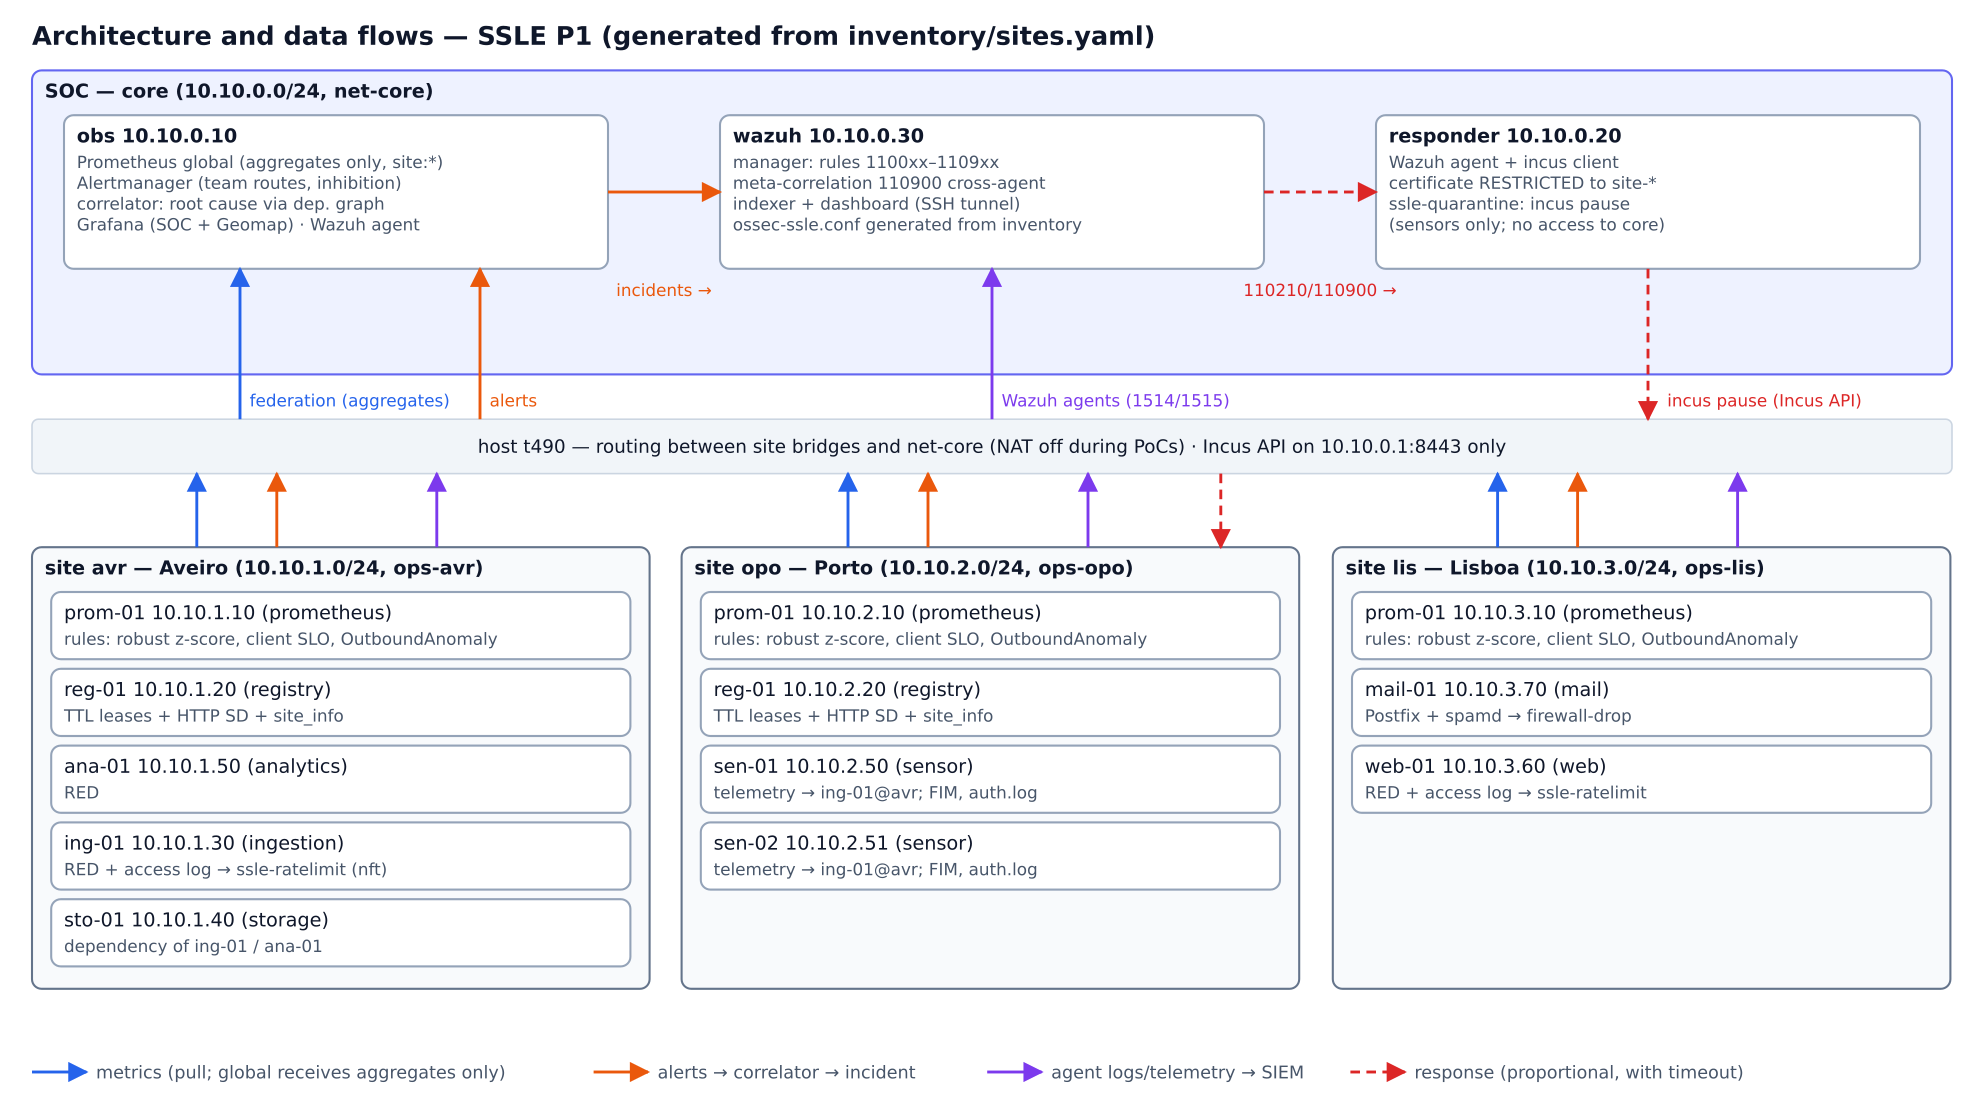
\includegraphics[width=\textwidth]{architecture.png}
  \caption{Architecture and data flows, generated from the inventory. Four flows: metrics
    (the global receives only aggregates), alerts $\to$ correlator $\to$ incident, agent logs
    $\to$ SIEM, and responses (dashed).}
  \label{fig:architecture}
\end{figure}

The entire infrastructure is \textbf{code}: a single inventory
(\texttt{inventory/sites.yaml}) generates the Incus projects and networks, containers,
Prometheus targets, the correlator's dependency graph, site registry configuration and
Grafana datasources. Adding an element or a site amounts to adding lines to the inventory
and re-running the idempotent deploy.

\begin{figure}[H]
  \centering
  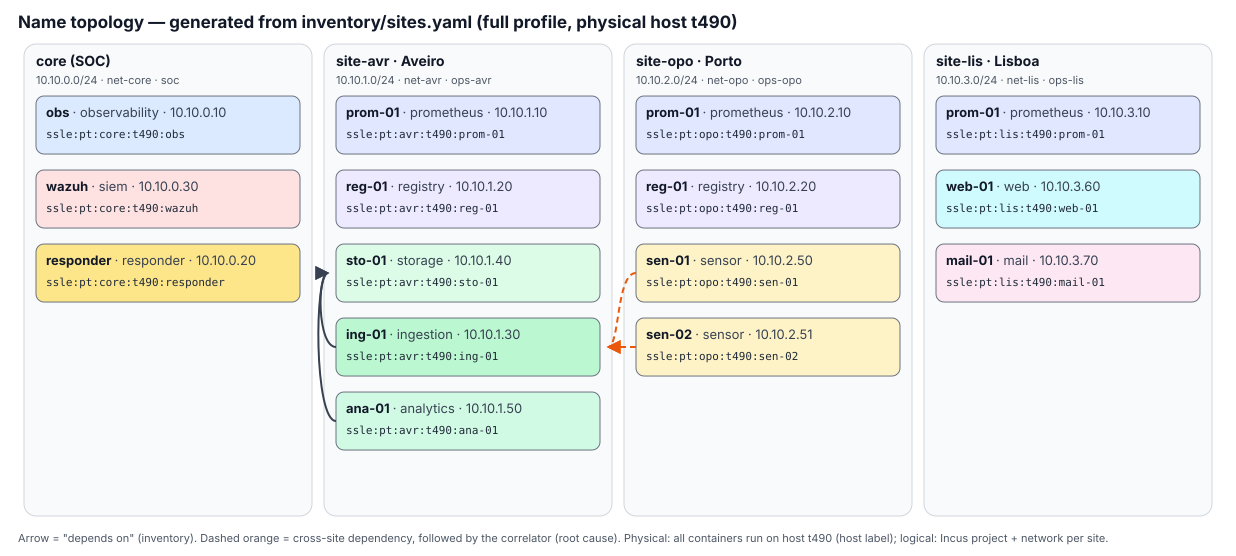
\includegraphics[width=0.85\textwidth]{topology.png}
  \caption{Name topology (full profile). One column per Incus project/network; each box
    holds the element's canonical identity; arrows are inventory dependencies, dashed arrows
    are cross-site dependencies the correlator follows.}
  \label{fig:topology}
\end{figure}

\begin{figure}[H]
  \centering
  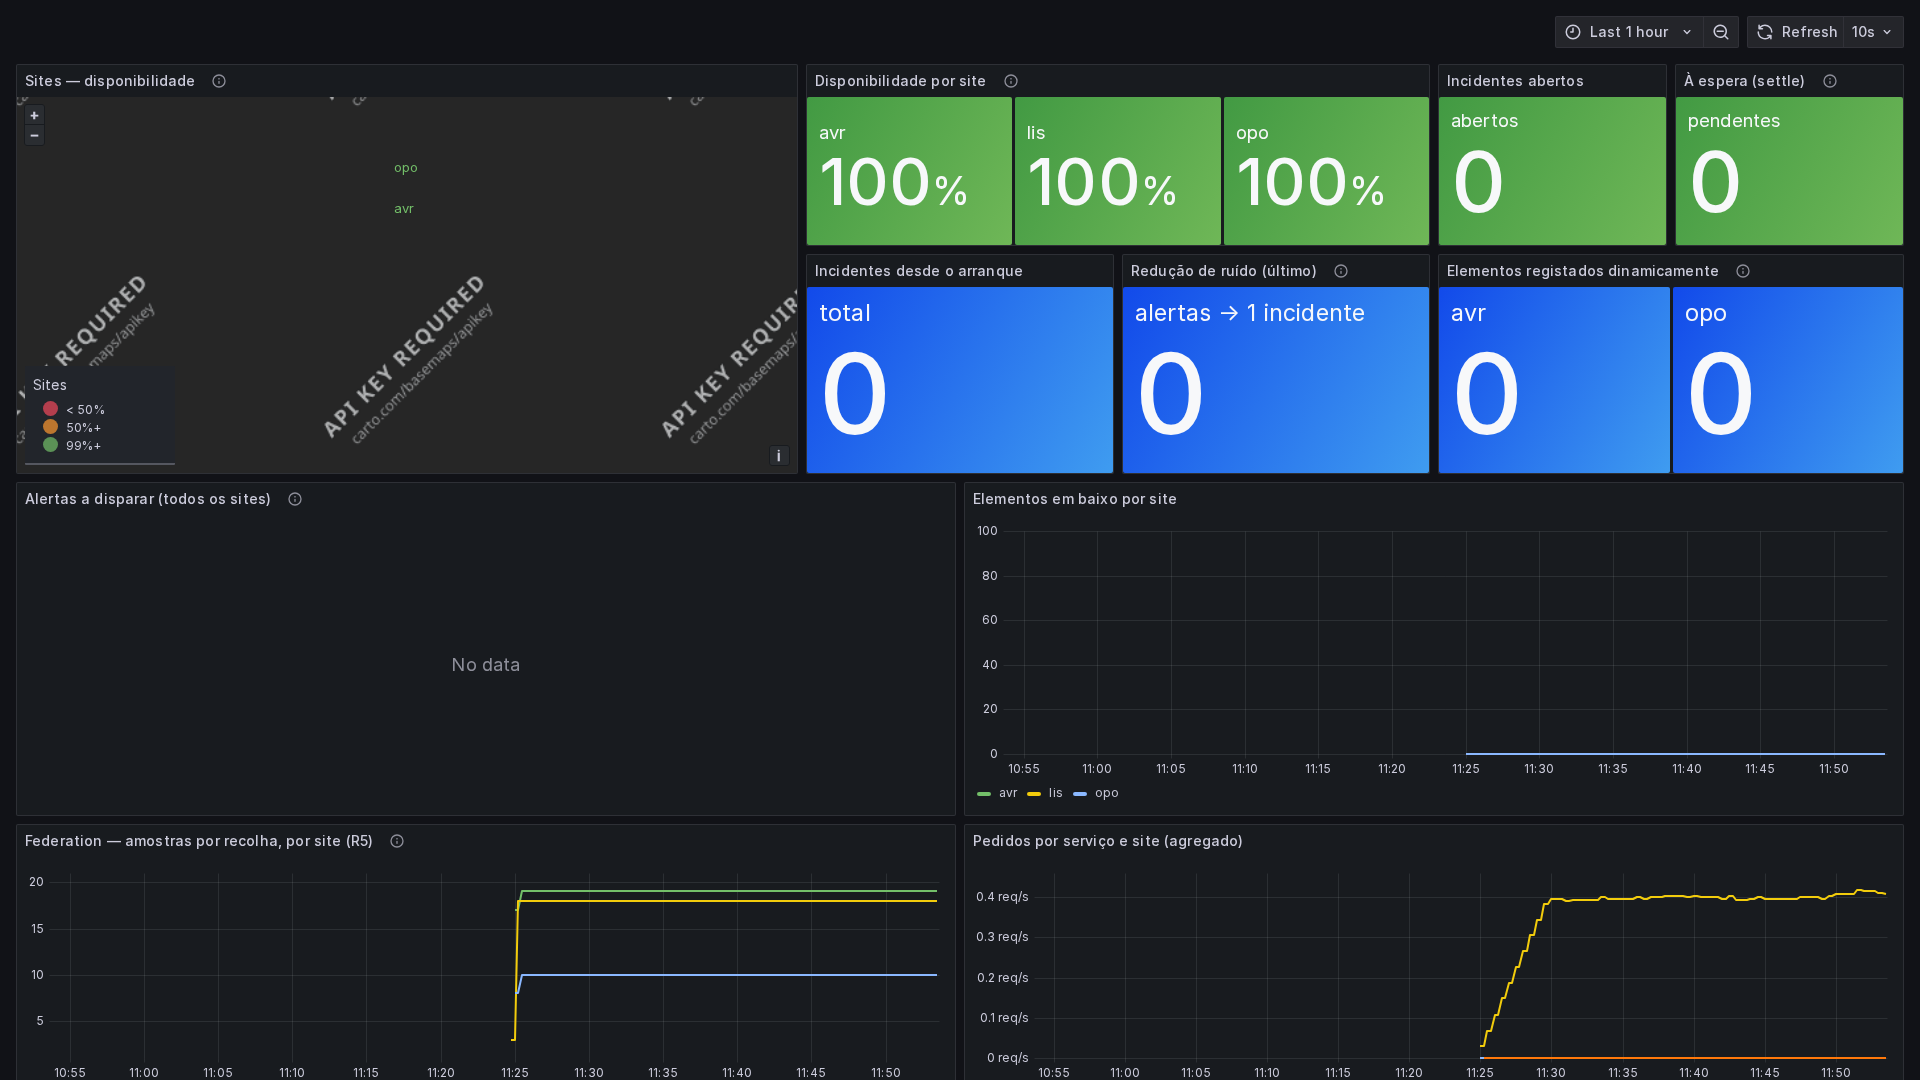
\includegraphics[width=\textwidth]{grafana-soc-live.png}
  \caption{SOC dashboard (live, T490, 22/11, a quiet 15~min): per-site availability, open
    incidents, settling alerts, federation cost per site, aggregated request rate and
    element-down history. The geomap places each site using coordinates from the inventory.
    The figures are rendered on the host with the same dashboards and the lab's Prometheus
    servers (\texttt{monitoring/grafana/shot-live.sh}); inside the lab, with NAT off, the base
    map does not load, only the markers.}
  \label{fig:soc-dashboard}
\end{figure}

\subsection{Identification and Registration}

Each element has a \textbf{canonical identity}
\texttt{ssle:<region>:<site>:<host>:<instance>}---for example,
\texttt{ssle:pt:avr:t490:ing-01}---used \textbf{identically} in Prometheus (labels
\texttt{region}, \texttt{site}, \texttt{host}, \texttt{instance\_name}, \texttt{role},
\texttt{team}, \texttt{project} and the \texttt{identity} annotation on each alert), in the
correlator and in Wazuh. The identity is hierarchical by design: the order
region $\to$ site $\to$ physical host $\to$ instance is the order an operator uses to narrow
down a fault.

Registration operates at two levels:

\begin{itemize}
  \item \textbf{Base fleet}---inventory elements, discovered by Prometheus via \texttt{file\_sd}
    generated at deploy time;
  \item \textbf{Dynamic elements}---a \textbf{per-site registry} (\texttt{reg-01}) that
    extends the lecture-2 service registry with time-limited leases renewed by the element
    itself (an element that dies disappears on its own after the TTL), authenticated writes
    via a per-site token generated at deploy, name/role/site/subnet validation, and refusal
    of identity claims from a mismatched IP. Prometheus discovers them via \textbf{HTTP SD}.
\end{itemize}

The two mechanisms do not overlap: HTTP~SD returns only dynamic elements. If the registry
fails, the base fleet remains monitored (fail-safe). The integration test, with a real
Prometheus~2.53.5, shows an out-of-inventory sensor appearing in the targets with the
identity labels and leaving them 9~s after dying (TTL of 10~s in the test).

\subsection{Physical, Logical and Geographic Location}

\begin{itemize}
  \item \textbf{Physical}---the \texttt{host} label identifies the machine running the
    container (\texttt{t490} in production, \texttt{mac-m2} in staging). The three sites are
    emulated on a single physical host, a limitation discussed in Section~\ref{sec:conclusions}.
  \item \textbf{Logical}---each site is an \textbf{Incus project} with its own bridge
    (\texttt{net-avr}/\allowbreak\texttt{10.10.1.0/24}, etc.)\ and DNS domain
    \texttt{<site>.ssle.lab}; the core sits on \texttt{net-core}
    (\texttt{10.10.0.0/24}). Quarantine is \texttt{incus~pause}: it freezes the
    container, preserving memory and disk for forensics.
  \item \textbf{Geographic}---latitude and longitude of each site are in the inventory,
    published by the site registry as \texttt{site\_info} and aggregated into
    \texttt{site:info:last}, which feeds the SOC dashboard map.
\end{itemize}

Delegation follows the site: each site has its own team (\texttt{team}), which routes alerts
in the Alertmanager; its own registry, which accepts only elements from its own site and
subnet; and its own Wazuh agent group with site-specific shared configuration.

\subsection{Hierarchical Monitoring}

Each site has its own Prometheus (\texttt{prom-01}, scrape interval 15~s) that evaluates
\textbf{locally} the availability and anomaly rules per instance and computes per-site
aggregates following the \texttt{level:metric:operations} convention. The \textbf{global
Prometheus} collects from each site via federation, at 30~s, \textbf{only} the aggregates
(\texttt{site.*:.*}), the \texttt{up} of each target and the active alerts---never the raw
time series. Detection stays close to the source, where temporal resolution exists, and the
SOC receives only the summary. Per-instance detail remains accessible in Grafana through a
per-site datasource, queried only on demand. The bandwidth savings (with and without
aggregation) are part of the evaluation (Section~\ref{sec:evaluation}).

\subsection{Detection and Correlation}

Anomaly detection uses \textbf{three independent layers}:

\begin{enumerate}
  \item \textbf{Relative}---\texttt{TrafficAnomaly}, a \textbf{robust z-score} of each
    instance's request rate against the last hour (median and interquartile range instead of
    mean and standard deviation). The mean/std version lets an attack ``contaminate'' the
    baseline, and a second attack within the same hour no longer fires. The unit test
    demonstrates this ($z = 39.6$ vs $\approx 2.0$) and the T1~PoC confirmed it with real
    traffic (Section~\ref{sec:t1});
  \item \textbf{Absolute, server-side}---\texttt{ServiceLatencyHigh}, the latency SLO
    ($p_{95} < 100$~ms) measured at the application;
  \item \textbf{Absolute, client-side}---\texttt{ClientLatencySLO} and
    \texttt{ClientUpstreamErrors}, the same SLO measured \textbf{by the sensors} when
    sending. This layer was added after the T1~PoC, which showed that the server does not
    see the queuing time before serving (Section~\ref{sec:t1}).
\end{enumerate}

Correlation has two stages. The Alertmanager groups and applies \textbf{topological
inhibition} within a host or site (\texttt{SiteUnreachable} silences the site's symptoms;
\texttt{ElementDown} silences the instance's symptoms). The \textbf{correlator} receives the
alerts and selects root causes over the \textbf{inventory dependency graph} via
\textbf{greedy set-cover}: it picks the alerting node that explains the most unexplained
symptoms (a node explains a symptom if the symptomatic element depends on it, directly or
transitively), removes them and repeats. The graph has no site boundaries, so the latency
felt by a Porto sensor is attributed to the Aveiro ingestion service. Two independent faults
yield two incidents, and each symptom belongs to exactly one incident. A \textbf{settle
window} of 30~s prevents emitting a root cause while related symptoms may still be arriving:
without it, a client symptom arriving first would make the sensor the root cause, which the
SIEM would interpret as a quarantine candidate. The ten tests cover these cases, including
the counterproof without stabilisation and the fields the SIEM uses (\texttt{srcip} = root
cause IP, \texttt{alert\_names}).

Each incident is a JSON line in \texttt{incidents.json} (root cause, affected elements,
sites, severity, originating alerts, noise reduction), which the Wazuh agent on \texttt{obs}
sends to the SIEM. This is the Prometheus~$\to$~Wazuh bridge (rules 110000--110099).

\subsection{SIEM and Response}

Wazuh (manager, indexer and dashboard) runs on the core. Each element has an agent enrolled
in two groups, the \textbf{site} group and the \textbf{role} group (\texttt{site-opo} +
\texttt{role-sensor}, etc.), with the same identity labels as Prometheus, carried in every
alert. The shared configuration of each group specifies what to collect: \texttt{auth.log}
and FIM on persistence directories for sensors, the access log of exposed services, the
\texttt{mail.log} of the MTA, the \texttt{incidents.json} of the correlator on \texttt{obs}
and a remote command listing TCP listening ports.

The project's rules occupy reserved ranges---\texttt{1100xx}~correlator,
\texttt{1101xx}~T1, \texttt{1102xx}~T2, \texttt{1103xx}~T3,
\texttt{1109xx}~meta-correlation---and are validated at two levels before deployment:

\begin{enumerate}
  \item \textbf{25 assertion-based cases} on the real \texttt{wazuh-analysisd}~4.14.10,
    with both positive and negative cases;
  \item \textbf{Integration with real agents}: manager and five \texttt{wazuh-agent}
    instances in Docker (including a Postfix with \texttt{spamd}), installed by the deploy
    scripts, from stimulus to response on the correct agent (34~checks).
\end{enumerate}

These two levels uncovered \textbf{17~defects} (2~fatal at load time, 7~caught by the
assertion cases, 8~only with real agents), and the live lab two more
(Section~\ref{sec:evaluation}). Of the~19, 16~were silent: the SIEM started,
the dashboard showed green, and the threat went undetected. For example: a second
\texttt{<ruleset>} that erased default lists; a composite rule over a level-0 rule whose
events the \texttt{analysisd} discards; cross-agent correlation requiring
\texttt{<global\_frequency/>} because composite-rule state is per-agent; and \texttt{ignore}
being per-rule rather than per-source.

\paragraph{Responses.}
The manager configuration (whitelist, lists, commands, responses) is \textbf{generated from
the inventory} and \textbf{merged} into \texttt{ossec.conf}, idempotently and with rollback
to the last known-good state if the manager rejects it. Responses are proportional and
reversible (all with \texttt{timeout}):

\begin{table}[H]
  \centering
  \caption{Active-response mapping.}
  \label{tab:responses}
  \small
  \begin{tabular}{@{}p{3.2cm}p{5cm}p{4.8cm}@{}}
    \toprule
    \textbf{Trigger} & \textbf{Response} & \textbf{Runs on} \\
    \midrule
    110100/101/110 (T1) & \texttt{ssle-ratelimit}: per-origin limit (nft) &
      The attacked service \\
    110210/110900 (T2/meta) & \texttt{ssle-quarantine}: \texttt{incus pause} of the sensor &
      \texttt{responder} (Incus cert restricted to \texttt{site-*}) \\
    110302/110900 (T3, meta) & \texttt{firewall-drop} of the origin &
      The attacked MTA (or service) \\
    \bottomrule
  \end{tabular}
\end{table}

The quarantine target is resolved via the fleet map generated from the inventory, never as
received in the alert, and the script refuses anything that is not a sensor in a site
project. For T1, the root cause is the \textbf{victim}, so the response rate-limits rather
than isolates.

\subsection{Infrastructure Decisions}

\begin{table}[H]
  \centering
  \caption{Key infrastructure decisions.}
  \label{tab:decisions}
  \begin{tabular}{@{}p{4cm}p{3cm}p{6.5cm}@{}}
    \toprule
    \textbf{Decision} & \textbf{Alternative} & \textbf{Rationale} \\
    \midrule
    Incus system containers, one project + network per site &
      VMs; Kubernetes &
      Site isolation and delegation at container cost; lecture scripts run identically inside \\
    T490 (x86\_64, 24\,GB) as production; Mac (arm64~VM) as staging &
      Everything on Mac &
      Wazuh (4--6\,GiB), three Prometheus, the fleet and $\geq$8\,GiB margin for load tests
      do not fit in 7.7\,GiB \\
    Single host update then \textbf{freeze} until demo &
      Continuous updates &
      Arch is rolling-release: a new kernel or Incus the day before is the biggest
      operational risk \\
    SOC stack via packages + systemd on \texttt{obs} &
      Docker Compose inside the container &
      Same path validated in staging, without nested containers \\
    NAT only during provisioning &
      Permanent NAT &
      With NAT, ingestion sees attacker and sensors with the same IP (the gateway), preventing
      per-origin responses and attack attribution \\
    \bottomrule
  \end{tabular}
\end{table}


%% ============================================================================
\section{Risk Management and Mitigation}
\label{sec:risk}
%% ============================================================================

\subsection{Threat Model, Assets and Attack Surface}

The threat model is that of the \textbf{remote attacker} from lecture~5: someone who reaches
the site networks (bridges \texttt{net-avr}, \texttt{net-opo}, \texttt{net-lis}) but has no
physical access to the hypervisor nor to the SOC network (\texttt{net-core}). Attacks on the
host itself and supply-chain attacks on the container images are deliberately excluded.

\begin{table}[H]
  \centering
  \caption{Assets and attack surface.}
  \label{tab:assets}
  \begin{tabular}{@{}p{2.5cm}lp{4cm}p{4cm}@{}}
    \toprule
    \textbf{Asset} & \textbf{Site} & \textbf{Exposed surface} & \textbf{Loss (CIA)} \\
    \midrule
    Ingestion \texttt{ing-01} & avr & HTTP \texttt{:8000} (\texttt{/ingest}, \texttt{/work}),
      \texttt{:9100} &
      \textbf{A}: single entry point for all sensors \\
    Sensors \texttt{sen-0x} & opo & \texttt{:8000}, \texttt{:9100}, management access &
      \textbf{I} of element $\to$ \textbf{A} of third parties (bots) \\
    MTA \texttt{mail-01} & lis & SMTP \texttt{:25} &
      \textbf{A} (queue, resources) and \textbf{C} (social engineering) \\
    Monitoring and SIEM & core & Wazuh 1514/1515, dashboard \texttt{:443}, Incus API \texttt{:8443} &
      \textbf{I} of detection itself---a blind SOC does not alarm \\
    \bottomrule
  \end{tabular}
\end{table}

The last row is the easiest to forget: the detection system is itself an asset. Hence the
dashboard and Grafana are reachable only via SSH tunnel, the Incus API listens only on the
core bridge, and the \texttt{responder}'s certificate is restricted to \texttt{site-*}
projects.

\subsection{Risk Matrix and Threat Selection}

Likelihood and impact on a qualitative 1--3 scale, for the seven threats from the assignment:

\begin{table}[H]
  \centering
  \caption{Risk matrix.}
  \label{tab:risk}
  \begin{tabular}{@{}lcccp{4.5cm}@{}}
    \toprule
    \textbf{Threat} & \textbf{Likelihood} & \textbf{Impact} & \textbf{Risk} & \textbf{Decision} \\
    \midrule
    Massive DoS/DDoS & 3 & 3 & \textbf{9} & $\checkmark$ T1 \\
    IoT fleet botnet & 2 & 3 & \textbf{6} & $\checkmark$ T2 \\
    Junk e-mail (spam) & 3 & 2 & \textbf{6} & $\checkmark$ T3 \\
    APT & 1 & 3 & 3 & Partially covered by T2 \\
    Fraud/social attacks & 2 & 2 & 4 & Social side of T3 (SPF/DKIM/DMARC, planned) \\
    Reputation systems & --- & --- & --- & Used as \textbf{defence} (CDB, RBL) \\
    Route/signal hijacking & 1 & 3 & 3 & Out of scope (would require BGP/FRR) \\
    \bottomrule
  \end{tabular}
\end{table}

The chosen trio covers the CIA triad and three detection families: metrics and anomalies (T1),
endpoint telemetry (T2) and application-content with reputation (T3). It also connects into a
single story: botnets are the typical origin of DDoS and
spam~\cite{kolias2017,antonakakis2017}, and this link is what meta-correlation rule~110900
looks for.

\subsection{Attack--Defence Trees}

Figures~\ref{fig:adtree-t1}--\ref{fig:adtree-t3} follow the notation of Kordy et~al.:
red ellipses for attacks, green rectangles for defences, an arc for conjunctive refinement
(AND) and a dashed edge for the countermeasure.

\begin{figure}[H]
  \centering
  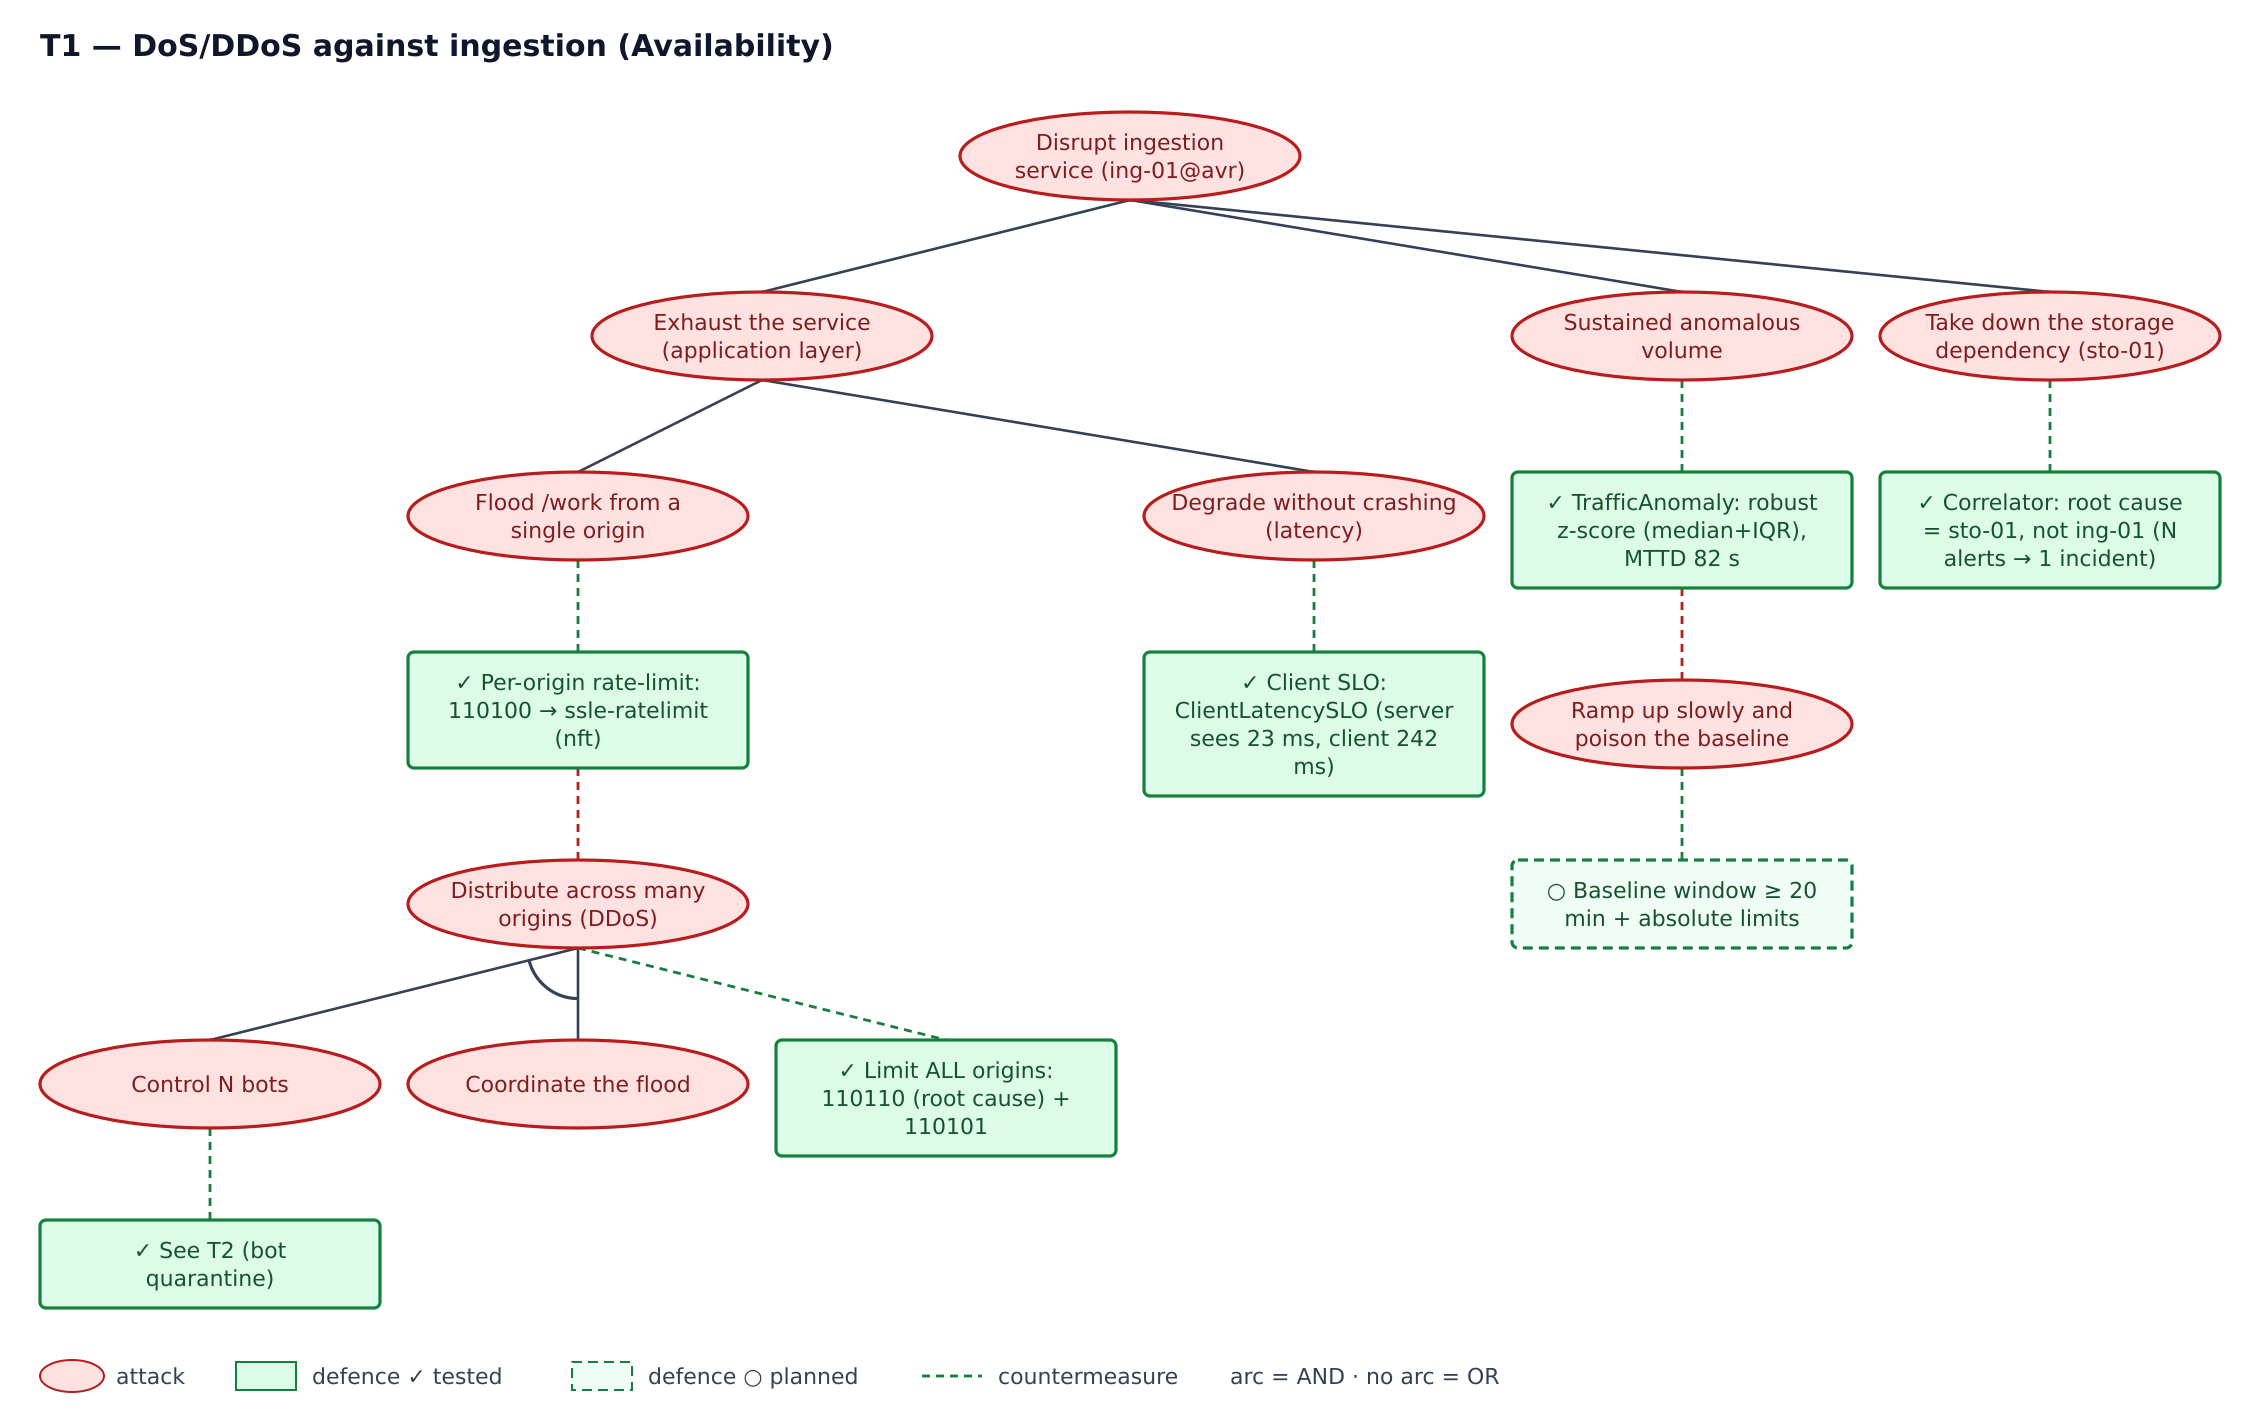
\includegraphics[width=\textwidth]{adtree-t1.png}
  \caption{ADTree for T1 (DoS/DDoS).}
  \label{fig:adtree-t1}
\end{figure}

\textbf{T1.} The longest chain is the application branch: the per-origin
rate-limit (rule~110100 $\to$ \texttt{ssle-ratelimit}) pushes the attacker to distribute
the load, an AND (control $N$~bots \textbf{and} coordinate them). The defence against the
distributed variant limits \textbf{each} origin when the correlator points to the service
itself as root cause (rule~110110). The ``take down the storage dependency'' node shows the value of
correlation: without it, the operator would look for the problem at \texttt{ing-01}, which
is only the symptom.

\begin{figure}[H]
  \centering
  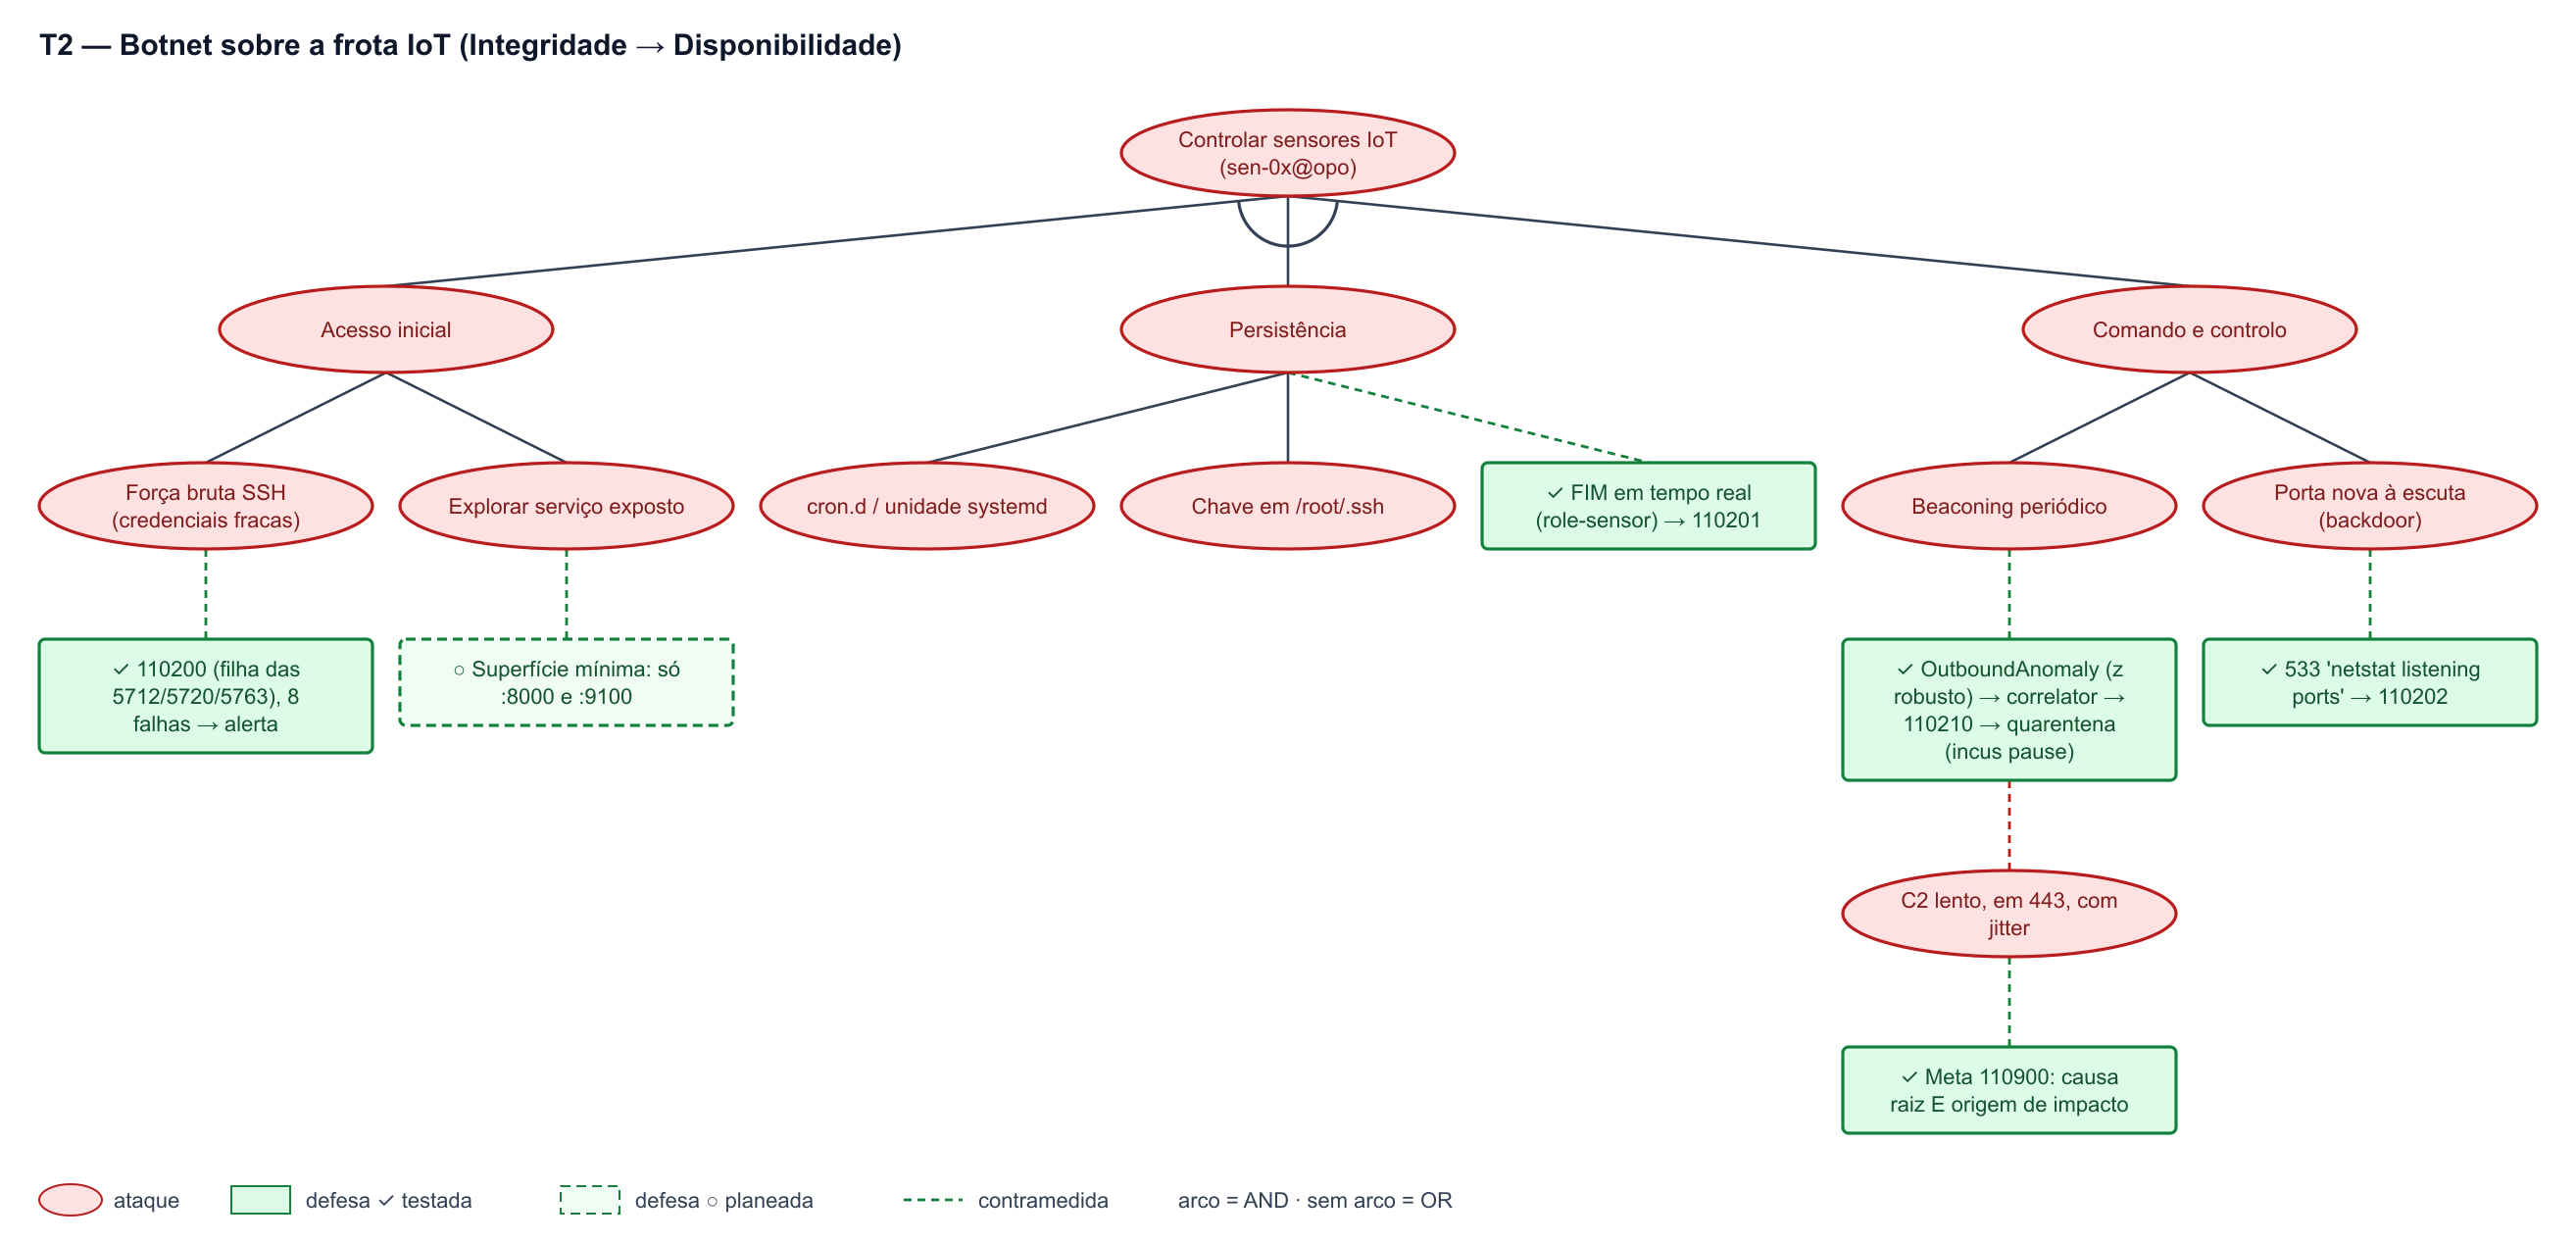
\includegraphics[width=\textwidth]{adtree-t2.png}
  \caption{ADTree for T2 (Botnet).}
  \label{fig:adtree-t2}
\end{figure}

\textbf{T2.} The root is an AND of three phases (initial access, persistence and C2). For
the attacker, all three must succeed; for the defender, breaking one suffices. This is the
formal argument for defence in depth: there is an independent detection per phase
(110200, 110201, 110202/110210). The most realistic counterattack is a slow C2, over 443
with jitter, that evades the traffic anomaly. The project's response is not to depend on a
single signal: rule~110900 joins ``this sensor is a root cause'' with ``this sensor is the
origin of an impact,'' even when each signal alone stays below the response threshold.

\begin{figure}[H]
  \centering
  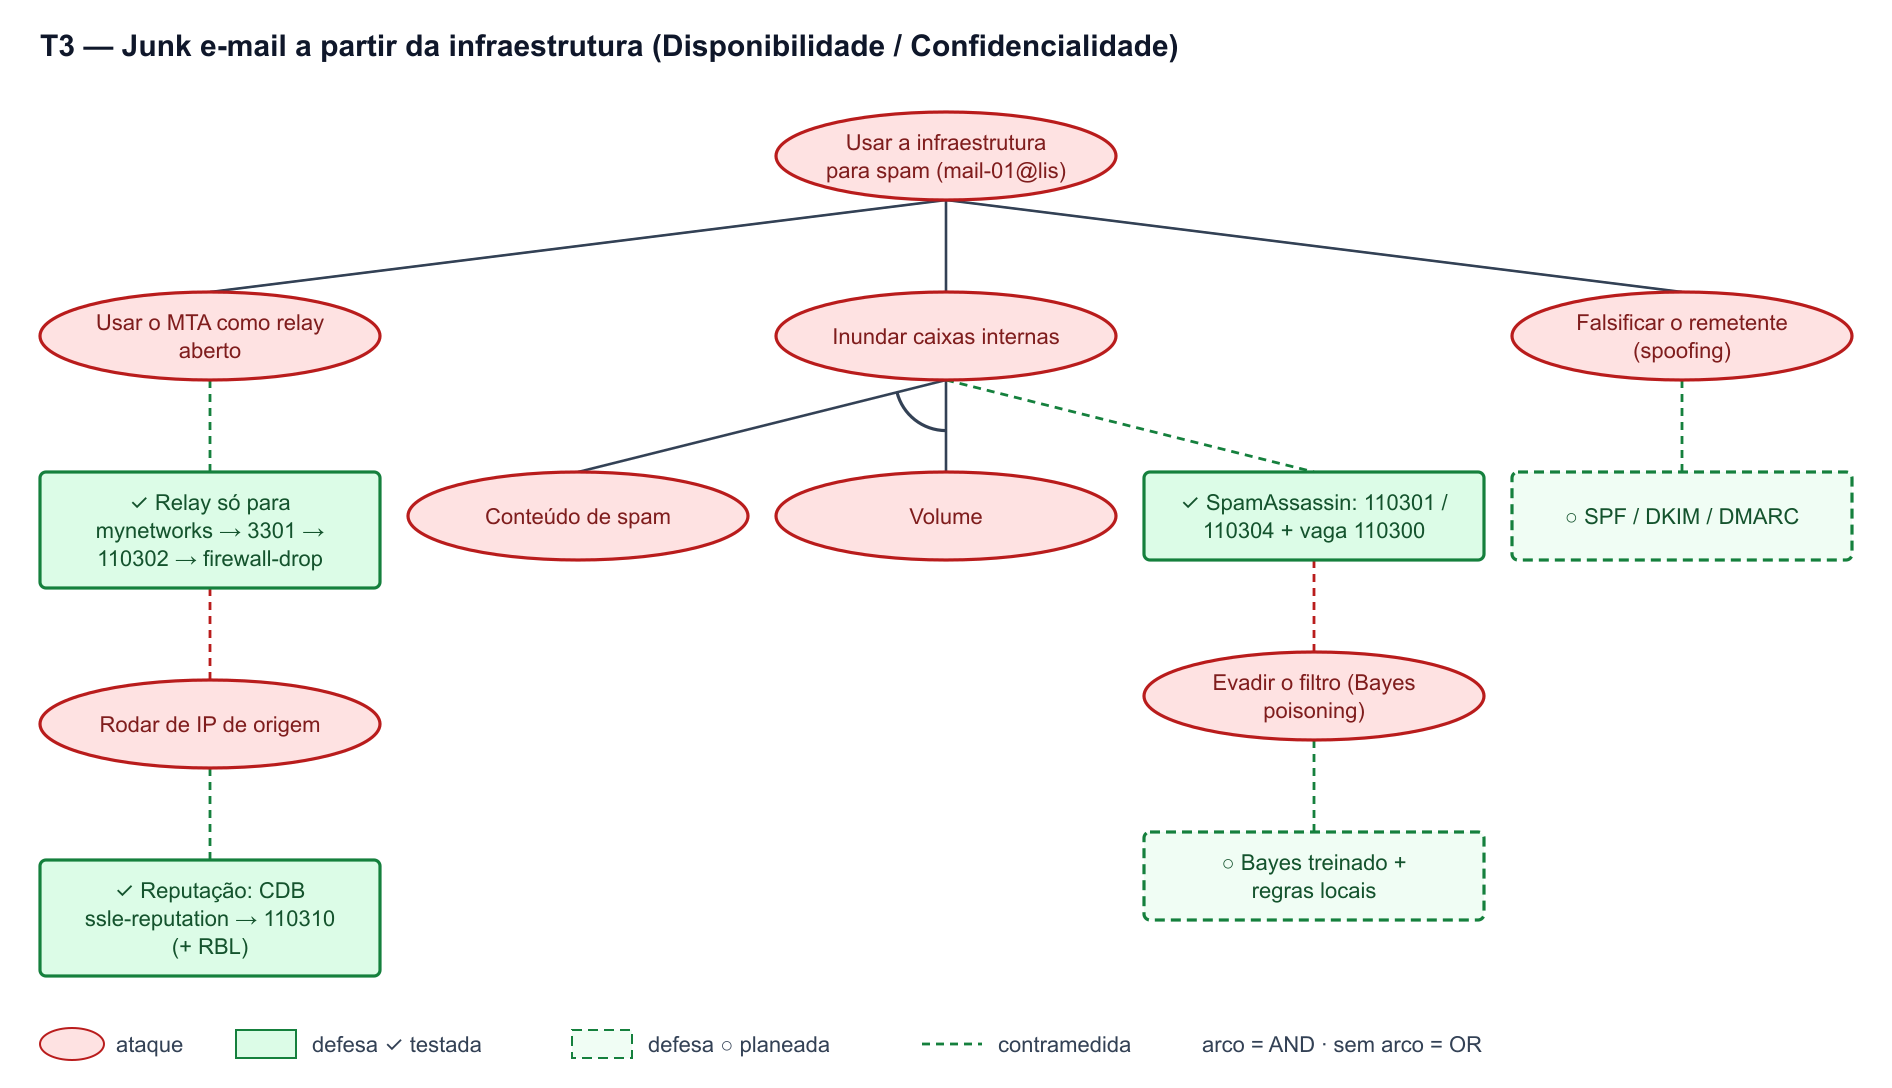
\includegraphics[width=\textwidth]{adtree-t3.png}
  \caption{ADTree for T3 (Spam).}
  \label{fig:adtree-t3}
\end{figure}

\textbf{T3.} Two independent routes (OR): use the MTA as a relay or flood internal
mailboxes. The second is an AND (content \textbf{and} volume), and therefore has two
separate detections: the SpamAssassin verdict (110301/110304) and the spam wave (110300).
Reputation (CDB) is the countermeasure against an attacker rotating IPs.
SPF/DKIM/DMARC remain as a planned countermeasure against spoofing.

\subsection{Mapping to CAPEC and ATT\&CK, and Controls Map}

\begin{table}[H]
  \centering
  \caption{Threat mapping to CAPEC, ATT\&CK and project controls.}
  \label{tab:controls}
  \small
  \begin{tabular}{@{}p{0.8cm}p{2.2cm}p{2.2cm}p{3.8cm}p{3cm}@{}}
    \toprule
    & \textbf{CAPEC} & \textbf{ATT\&CK} & \textbf{Detection} & \textbf{Response} \\
    \midrule
    T1 & 210$\to$\textbf{125} Flooding & T1499.003 &
      \texttt{TrafficAnomaly} (robust z); \texttt{ClientLatencySLO}; 110100/101/110 &
      \texttt{ssle-ratelimit} (nft, 300\,s) \\
    T2 & 112 $\to$ \textbf{49} Password Brute Forcing & T1110, T1053.003, T1543.002, T1571 &
      Wazuh 110200/110201/110202; correlator $\to$ 110210 &
      \texttt{ssle-quarantine} (\texttt{incus pause}, 600\,s timeout) \\
    T3 & 210 & T1496, T1534 &
      Wazuh 110300--110310 (spamd, Postfix, CDB) &
      \texttt{firewall-drop} (600\,s), reputation \\
    Meta & --- & --- &
      110900 (\texttt{if\_group} + \texttt{if\_matched\_group} + \texttt{same\_source\_ip}) &
      Quarantine of the origin \\
    \bottomrule
  \end{tabular}
\end{table}

Table~\ref{tab:mitre-rules} maps each detection rule in
\texttt{local\_rules.xml} to its MITRE ATT\&CK technique, as tagged in the XML
source (\texttt{<mitre><id>...</id></mitre>}).

\begin{table}[H]
  \centering
  \caption{MITRE ATT\&CK tags in Wazuh custom rules.}
  \label{tab:mitre-rules}
  \small
  \begin{tabular}{@{}llll@{}}
    \toprule
    \textbf{Rule} & \textbf{Threat} & \textbf{ATT\&CK ID} & \textbf{Technique} \\
    \midrule
    110100 & T1 & T1499.003 & Application Exhaustion Flood \\
    110101 & T1 & T1499.003 & Application Exhaustion Flood \\
    110110 & T1 & T1499.003 & Application Exhaustion Flood \\
    110200 & T2 & T1110    & Brute Force \\
    110201 & T2 & T1053.003, T1543.002 & Scheduled Task / Systemd \\
    110202 & T2 & T1571    & Non-Standard Port \\
    110210 & T2 & T1071    & Application Layer Protocol \\
    110300 & T3 & T1496    & Resource Hijacking \\
    110301 & T3 & T1534    & Internal Spearphishing \\
    110302 & T3 & T1496    & Resource Hijacking \\
    110304 & T3 & T1534    & Internal Spearphishing \\
    110900 & Meta & T1071, T1499 & App.\ Layer Protocol + DoS \\
    \bottomrule
  \end{tabular}
\end{table}

The spam rules are deliberately \emph{not} tagged T1566 (Phishing). T1566 is
\textbf{initial access} from outside, seen by whoever receives the mail; in T3 the sender is
an element of our own fleet that is already compromised (the T2~bot). Its abuse of the MTA
to emit volume or to relay outwards consumes our resources and reputation, which is
\textbf{T1496} (Resource Hijacking: 110300, 110302). Its messages to the domain's own
mailboxes come from inside the organisation, which ATT\&CK models as \textbf{T1534}
(Internal Spearphishing: 110301, 110304).

Common principles: all responses are \textbf{proportional} (limit before blocking, pause
instead of deleting), \textbf{reversible} (\texttt{timeout} and automatic \texttt{delete}),
\textbf{with an explicit target} (resolved from the fleet map, never used as received in the
alert) and \textbf{logged} (\texttt{active-responses.log}). They also have a SOC whitelist:
the response never turns against the monitoring itself.


%% ============================================================================
\section{Threat Analysis}
\label{sec:threats}
%% ============================================================================

\subsection{Threat 1 --- Denial of Service (Availability)}
\label{sec:t1}

\subsubsection{Description}

Application-layer denial of service (layer~7): concurrent requests to the most expensive
endpoint of the ingestion service exhaust the available CPU time for serving legitimate
clients. On the three axes from lecture~7: application layer, single origin (the distributed
variant uses clients on multiple sites) and constant pattern during a fixed window. In CIA,
it attacks \textbf{availability}.

\subsubsection{Relevance}

\texttt{ing-01} is the entry point for \textbf{all} sensors---a single point of failure. If
ingestion slows down, the telemetry from another site is delayed or lost without any sensor
being faulty. This is the scenario where an operator without correlation would look for the
problem in the wrong place. At scale, the origin is distributed and spans multiple sites,
requiring per-instance detection and cross-site correlation.

\subsubsection{Exploitation / PoC}

A \textbf{limited, fixed-duration} stimulus, only on the lab's internal networks:
20~concurrent \texttt{curl} cycles for 120~s against the \texttt{/work} endpoint of
\texttt{ing-01}, against a baseline of 0.2--0.4~requests/s generated by the sensors. The
stimulus (script and parameters) is the same in every run, but the load it
\textbf{delivers} is not: ${\sim}160$~requests/s in staging, where there was no response,
and ${\sim}21$~requests/s on the T490 (Table~\ref{tab:t1-results}), about $7\times$ less.
On the T490 the service itself is slower (server $p_{95}$ of 151--495~ms against 23~ms) and
serves only ${\sim}20$ \texttt{/work} requests/s---run~13 served 17~requests/s before any
limit was in place---and the per-origin limiter under test, active a few seconds into each
run at 20~new connections/s, binds at the same level (it dropped 1\,940 connection attempts
in run~10). Each run is measured by a script that records the stimulus start/end timestamps
and extracts the metrics from the \textbf{sources} (the \texttt{ALERTS} series, sensor
metrics and the correlator's \texttt{incidents.json}), not from a stopwatch.

\subsubsection{Metrics}

\begin{table}[H]
  \centering
  \caption{T1 measurement signals.}
  \small
  \begin{tabular}{@{}p{2.2cm}p{5.8cm}p{5.5cm}@{}}
    \toprule
    \textbf{Signal} & \textbf{Series} & \textbf{Use} \\
    \midrule
    Rate (R of RED) & \texttt{instance:http\_requests:rate1m} &
      Input to robust z-score (\texttt{TrafficAnomaly}) \\
    Server latency (D) & \texttt{instance:http\_request\_\allowbreak duration\_seconds:p95\_1m} &
      100\,ms SLO (\texttt{ServiceLatencyHigh}) \\
    \textbf{Client} latency & \texttt{instance:ssle\_sensor\_\allowbreak upstream\_duration\_seconds:\allowbreak p95\_1m} &
      Client-side SLO (\texttt{ClientLatencySLO}); defines \textbf{recovery} \\
    Lost readings & \texttt{ssle\_sensor\_readings\_total\allowbreak\{result="error"\}} &
      Damage to the legitimate fleet \\
    SOC arrival & \texttt{incidents.json} (timestamp, root cause) &
      End-to-end MTTD \\
    \bottomrule
  \end{tabular}
\end{table}

\textbf{MTTD} = first timestamp with the rule in \emph{firing} $-$ stimulus start.
\textbf{Recovery} = last timestamp with the client's $p_{95}$ above the SLO $-$ stimulus end.

\subsubsection{Detection and Response Results}

\begin{table}[H]
  \centering
  \caption{T1 results: staging control group vs.\ T490 with SIEM response.}
  \label{tab:t1-results}
  \small
  \begin{tabular}{@{}p{2.8cm}p{4.8cm}p{4.8cm}@{}}
    \toprule
    & \textbf{Control group} (staging, no response, 3~runs) &
      \textbf{T490 with SIEM response} (6~runs) \\
    \midrule
    Delivered load (peak) &
      $160.1 \pm 2.2$ requests/s &
      $21.5 \pm 1.1$ requests/s (bound by the service and the limiter) \\
    Detection \texttt{Traffic\-Anomaly} &
      MTTD $81.7 \pm 2.9$\,s (3/3) &
      MTTD $81.2 \pm 5.1$\,s (6/6) \\
    Mean/std counterproof &
      would fire in 1/3 & would fire in 3/6 \\
    \texttt{Service\-Latency\-High} (server SLO) &
      \textbf{0/3} & 5/6, never before the client SLO \\
    \texttt{Client\-Latency\-SLO} &
      3/3 retroactively ($T_0 + 80$\,s) & 6/6, MTTD $76.2 \pm 4.2$\,s \\
    \textbf{SIEM response} (110100 $\to$ nft) &
      --- & ${\sim}6$\,s (active in all runs) \\
    SOC incident (correlator) &
      MTTD $92.9 \pm 0.1$\,s (3/3, root cause \texttt{ing-01}) &
      MTTD $120.2 \pm 7.4$\,s (6/6, root cause \texttt{ing-01}) \\
    Dropped packets (nft) &
      --- & 597--1\,098 per run (runs 7--9) \\
    Lost readings &
      \textbf{0} & \textbf{0} \\
    Recovery after stimulus &
      45.0\,s & $43.4 \pm 11.0$\,s \\
    \bottomrule
  \end{tabular}
\end{table}

The SIEM response (\texttt{ssle-ratelimit}, rule~110100: $\geq 100$ requests/10\,s from the
same origin $\to$ nft at 20~conn/s) activates in ${\sim}6$\,s---more than ten times faster
than metric-based detection (${\sim}80$\,s). The nft rule creates a per-origin set at
20~conn/s (burst~40), dropping excess without affecting the legitimate sensors
(0.2~conn/s). Rule~110110 (correlator: root cause in an exposed service) fires ${\sim}2$\,min
later and should extend the limit to \textbf{all} origins. In runs~4--10 it was a silent no-op
(the 18th defect, found by the multi-origin run below); with a single origin this did not change
the outcome, because 110100 had already limited that origin.

\paragraph{Re-run and distributed variant (T490, 22/11).}
Run~10 repeated the single-origin stimulus (Figure~\ref{fig:t1-attack}): \texttt{TrafficAnomaly}
MTTD 79.6\,s, SIEM response 1.6\,s (1\,940~packets dropped), SOC incident at 124.7\,s with
root cause \texttt{ing-01}, 0~lost readings---within the spread of runs~4--9. The distributed variant splits the same
21~clients across \textbf{three origins on three sites} (7~each, 240\,s): the hypervisor on
\texttt{net-avr}, \texttt{sen-02} (\texttt{opo}) and \texttt{web-01} (\texttt{lis}).

\begin{table}[H]
  \centering
  \caption{T1 with three origins (evidence in \texttt{threats/t1-ddos/evidence-ddos/}).}
  \label{tab:t1-ddos}
  \small
  \begin{tabular}{@{}p{3.6cm}p{3.4cm}p{3cm}p{3cm}@{}}
    \toprule
    & \textbf{Run 11} (before the fix) & \textbf{Run 12} (after) & \textbf{Run 13} (after) \\
    \midrule
    Requests served (mean) & 60\,req/s & 17\,req/s & 21\,req/s \\
    \texttt{TrafficAnomaly} MTTD & 79.9\,s & 79.7\,s & 79.1\,s \\
    SOC incident (root cause) & 124.0\,s (\texttt{ing-01}) & 115.1\,s (\texttt{ing-01}) & 120.5\,s (\texttt{ing-01}) \\
    Per-origin limit (110100) & host +3.9\,s, \texttt{sen-02} +124.9\,s & \texttt{sen-02} +20.7\,s & host +175.1\,s \\
    ``All origins'' (110101/110110) & \textbf{never engaged} & +20.7\,s (110101) & +120.1\,s (110110) \\
    Attack origins with a bucket & 2/3 (\texttt{web-01} never) & 3/3 & 3/3 \\
    Packets dropped & 25 & 0 & 0 \\
    Client $p_{95}$ max / lost readings & 600\,ms / 0 & 2\,369\,ms / 0 & 2\,367\,ms / 0 \\
    \bottomrule
  \end{tabular}
\end{table}

Detection and correlation do not depend on how the load is spread: MTTD stays at ${\sim}80$\,s
and the SOC incident points to \texttt{ing-01} in all three runs. The response did depend on it.
In run~11, 110101 ($\geq 300$ requests/10\,s in total) fired 4\,s into the attack and 110110 at
124\,s, but neither engaged: the per-origin rule, at one origin per minute (its \texttt{ignore}
is per rule), limited the hypervisor and \texttt{sen-02}, and \texttt{web-01} was never limited.
The cause: 110100 always puts the attacker's IP in the
\texttt{nft} interval set first, and the ``all origins'' element \texttt{0.0.0.0/0} overlaps
it, so \texttt{nft} refused it; the script stopped before logging, and \texttt{wazuh-execd},
which had already registered the key, answered ``already active'' to every later alert. It had
been silently inert since 12/11. After the fix (a separate set for the ``all'' mode, a
regression test, and every \texttt{nft} failure logged), every origin, attacker or legitimate,
gets its own bucket (runs~12--13).

That is also the limit of this defence. Each of the three origins stayed below 20~new
connections/s, so in runs~12--13 the limiter dropped \textbf{nothing} while the client
$p_{95}$ reached 2.4\,s: per-origin limiting cannot stop an attack spread below the per-origin
threshold. It raises the attacker's cost---the ``control $N$ bots \textbf{and} coordinate
them'' branch of the ADTree---but containing it needs aggregate admission control (a global
limit or fast 503s at the service) or a second replica (Section~\ref{sec:conclusions}). The
service throughput itself also varied between runs (60~req/s in run~11, 17--24 in runs~12--13
and ${\sim}21$ in the single-origin runs); the limiter was not the cause---run~13 served
17~req/s in its first 75\,s, before any limit was in place---and on a shared host we could not
isolate it, so the result we claim from these runs is the timing of detection and response,
not the impact. Finally, \texttt{sen-02}, as an attack origin, raised \texttt{OutboundAnomaly};
the correlator explained it as a symptom of \texttt{ing-01}, on which \texttt{sen-02} depends,
so a bot attacking its own upstream service is not quarantined by 110210.

\begin{figure}[H]
  \centering
  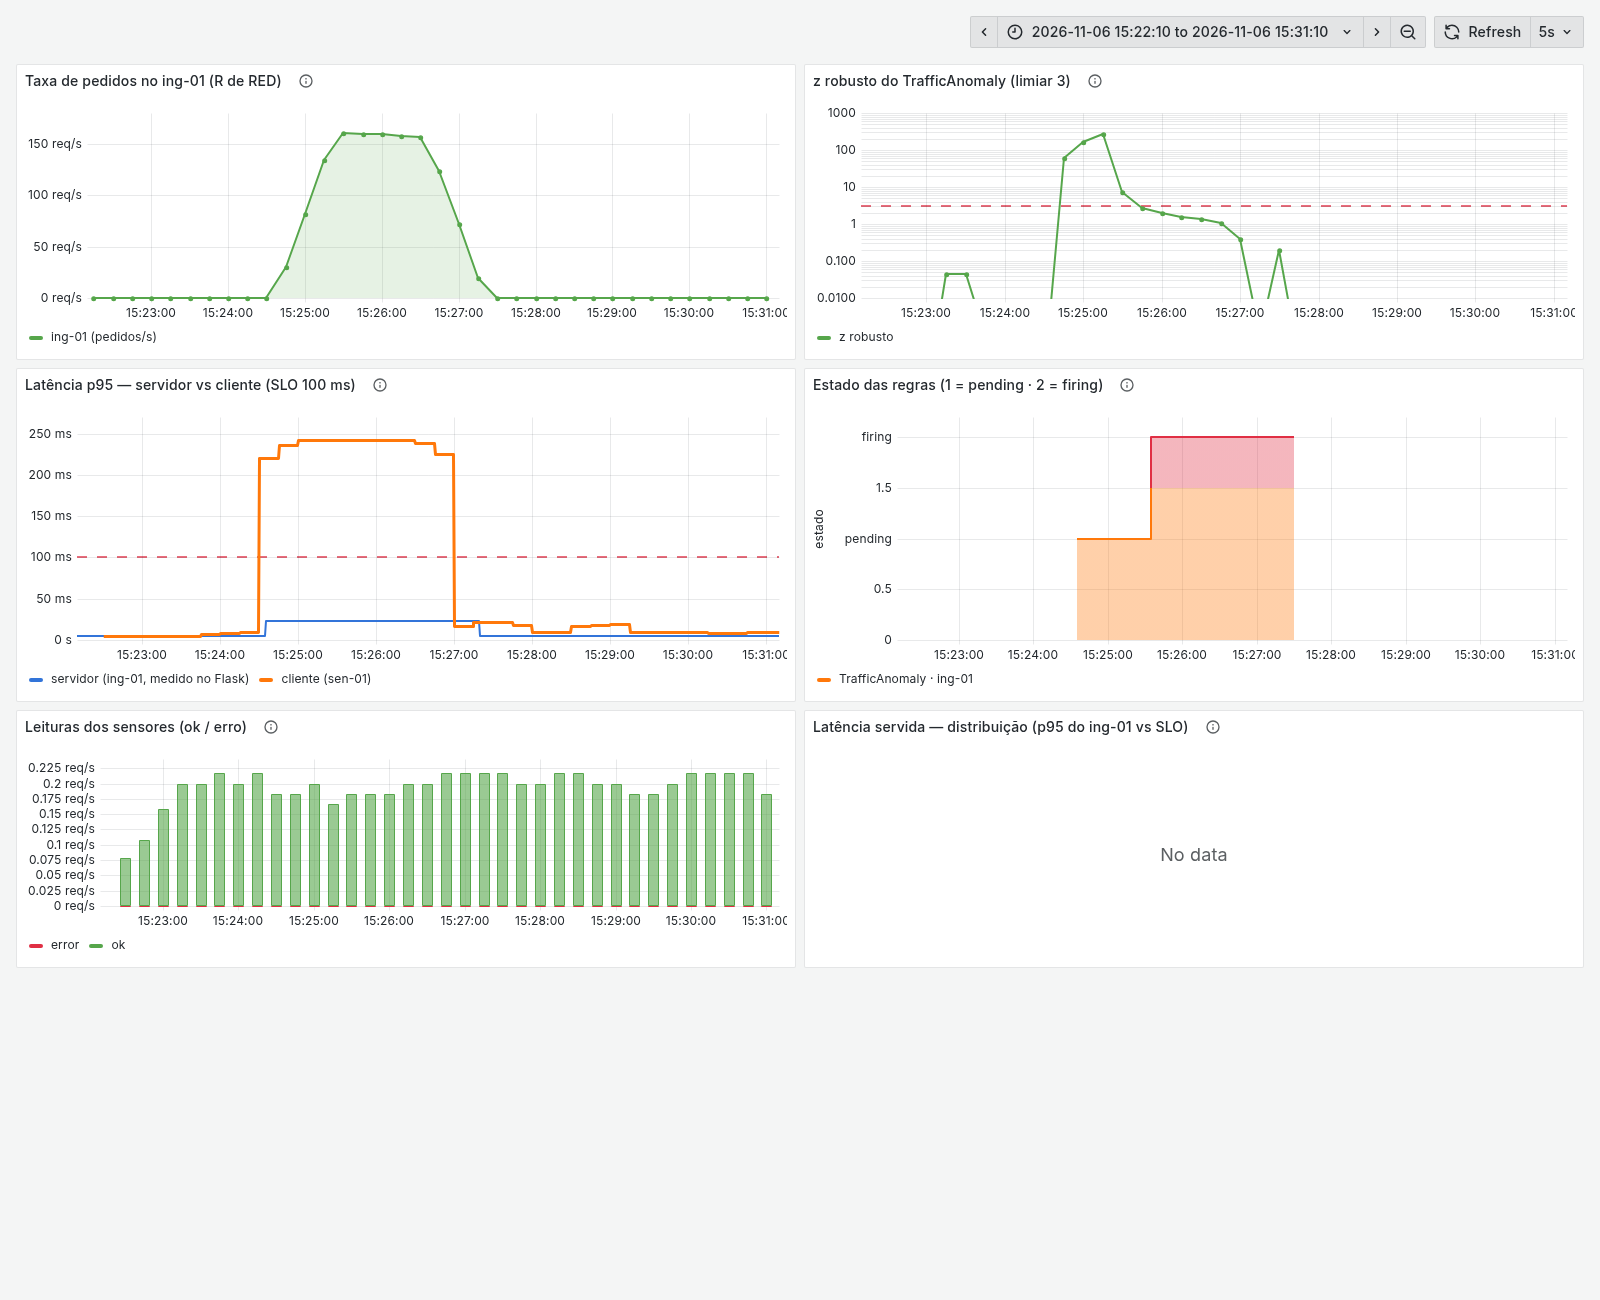
\includegraphics[width=\textwidth]{t1-replay-run1-dashboard.png}
  \caption{T1 run~1 on the \texttt{ssle-t1} dashboard: request rate at \texttt{ing-01},
    robust z-score (threshold~3), server latency (blue) vs.\ client latency (orange) with
    SLO, \texttt{TrafficAnomaly} state (pending $\to$ firing) and sensor readings. Replay
    from staging evidence of 06/11.}
  \label{fig:t1-dashboard}
\end{figure}

\begin{figure}[H]
  \centering
  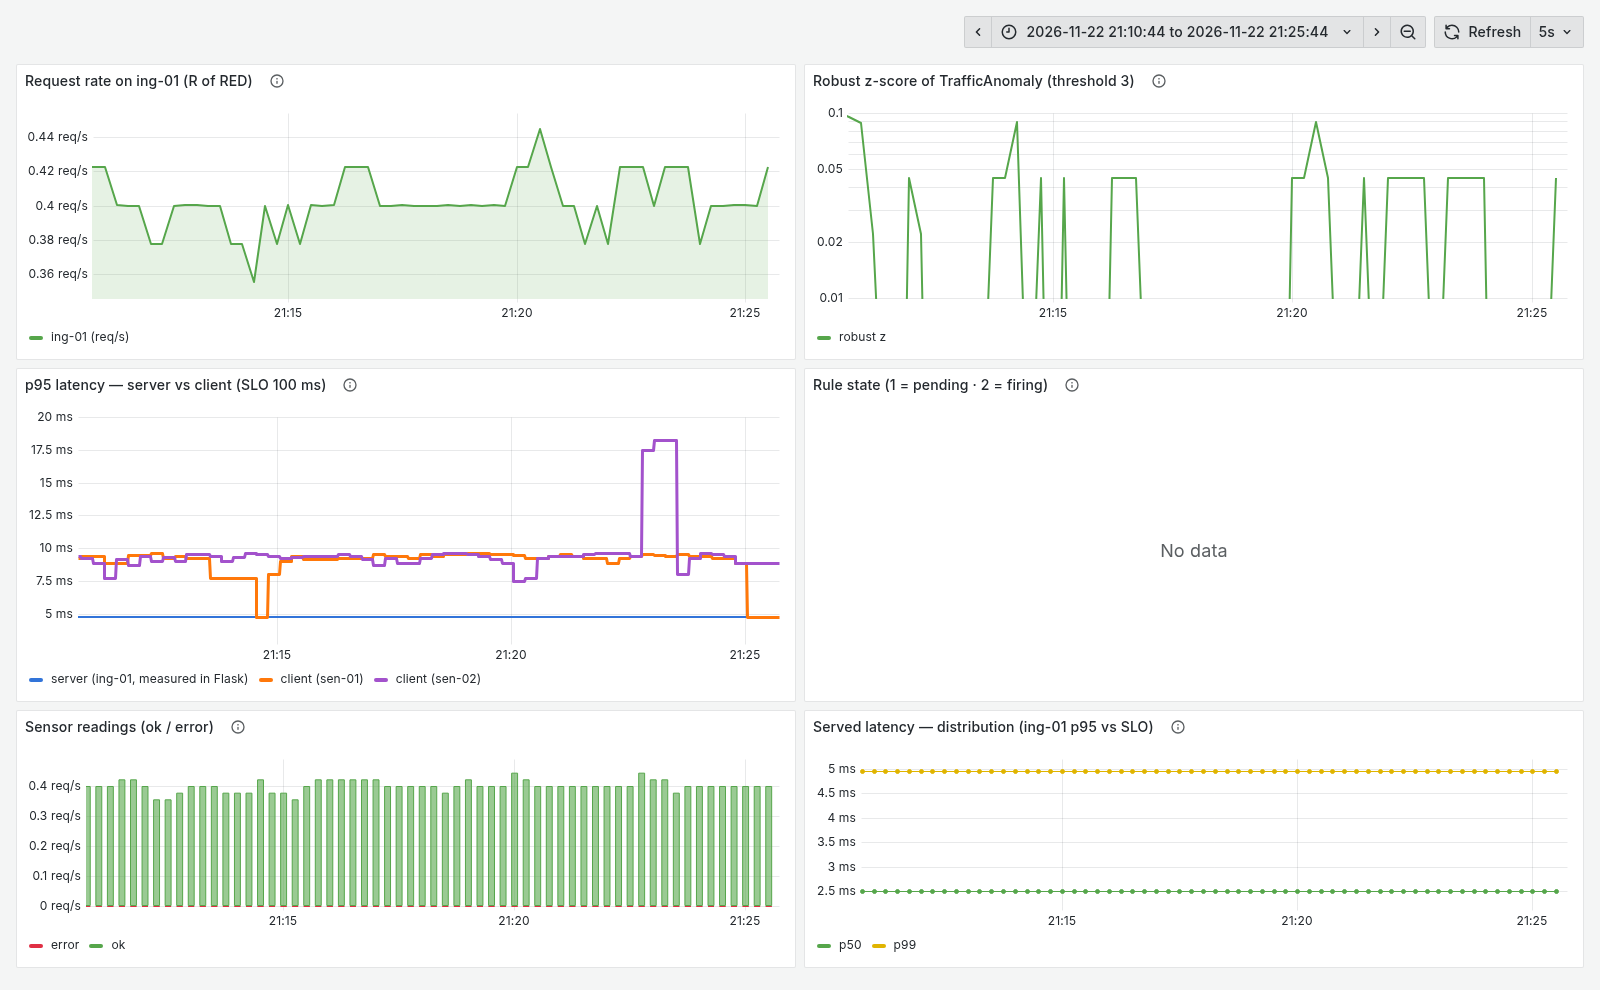
\includegraphics[width=\textwidth]{grafana-t1-live.png}
  \caption{T1 dashboard (live, T490, 22/11, the 15~min before run~10): request rate
    ${\sim}0.4$\,req/s from two sensors, robust z-score $< 0.1$ (no anomaly), client latency
    under 20\,ms against the 100\,ms SLO, and zero errors. This is the steady state before an
    attack.}
  \label{fig:t1-live}
\end{figure}

\begin{figure}[H]
  \centering
  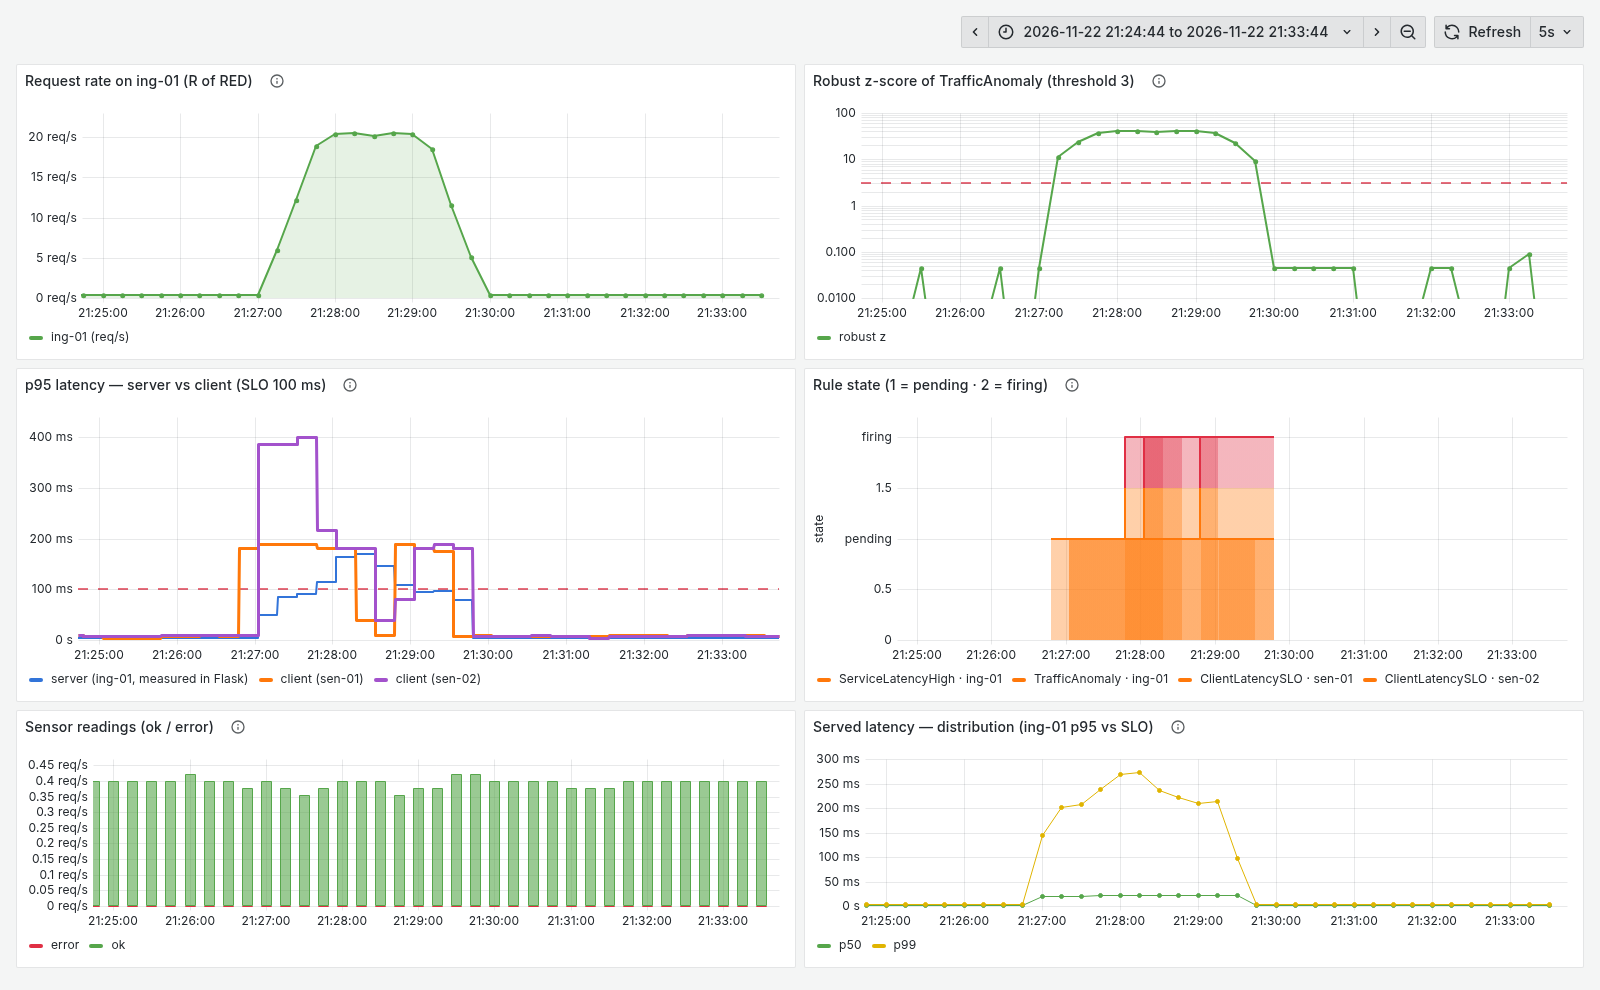
\includegraphics[width=\textwidth]{grafana-t1-attack.png}
  \caption{T1 run~10 (live, T490, 22/11): the request rate rises from the baseline to
    ${\sim}20$\,req/s (the service's capacity on the T490; \texttt{ssle-ratelimit} is active
    ${\sim}2$\,s into the run);
    the robust z-score crosses the threshold~3; the client $p_{95}$ (\texttt{sen-01} orange, \texttt{sen-02} purple) reaches ${\sim}400$\,ms
    against ${\sim}170$\,ms on the server (blue). Three rules fire, as four alert instances
    (orange pending, red firing):
    \texttt{TrafficAnomaly} and \texttt{ServiceLatencyHigh} on \texttt{ing-01}, and
    \texttt{ClientLatencySLO} on each of the two sensors.}
  \label{fig:t1-attack}
\end{figure}

\subsubsection{Post-mortem}

\paragraph{What worked.} The robust z-score detected all 9~runs and the
correlator opened \textbf{one} incident per run with the correct root cause. The live
counterproof confirmed what the unit test predicted: with mean/std, the first attack inflates
the standard deviation and later attacks within the same hour often \textbf{go undetected}.
An attacker repeating the attack would gain invisibility. The mean/std counterproof would
have missed 5 of the 9~runs: 2 of 3 in staging (max $z = 3.3$ and 2.8 in runs~2 and~3) and
3 of 6 on the T490 (max $z = 3.6$, 3.5 and 2.9 in runs~6, 8 and~9).

\paragraph{What did not work, and the lesson.}
In staging, the SLO measured \textbf{on the server} failed all three runs: the application
measured 23~ms while the client waited 242~ms. The server's histogram starts counting when the
request is already being served, and the queue \textbf{before} that (accepting the
connection, obtaining a thread, contending the interpreter with 20~expensive requests) is
invisible---and that queue is what the client feels. On the T490 the server SLO did fire in
5 of 6~runs, because there the service itself slowed down (server $p_{95}$ of 151--495~ms),
but it still under-reported the impact (client $p_{95}$ of 216--2\,200~ms), never fired
before the client-side rule (up to 60~s later in runs~4--5) and missed run~6 entirely.
\textbf{A latency SLO must be measured on the client side.} The fix is the third detection
layer: over the staging evidence it would fire in all three runs, and live on the T490 it
fired in all six.

\paragraph{Weaknesses found.}
\begin{enumerate}
  \item \textbf{NAT between sites} hides the attack origin (see Responses above).
  \item \textbf{Correlation limited to site} (fixed): the Porto sensor's symptom would open a
    second incident with the wrong root cause. The correlator now follows the graph across sites.
  \item \textbf{Risk introduced by the previous fix} (fixed): if the client symptom arrived
    first, the sensor would be identified as the root cause and the SIEM would treat it as a
    quarantine candidate---isolating a legitimate sensor during a DoS on the server. The
    settle window prevents this, at the cost of up to 30\,s in SOC MTTD.
  \item \textbf{Legitimate crowd or attack?} With the minimum dispersion of the rule, a
    legitimate fleet expansion would also trigger. Distinguishing the two would require a
    third signal (5xx error rate), which the Flask development server does not produce under
    load (it queues instead of refusing).
  \item \textbf{The ``all origins'' response never engaged} (fixed, 22/11): silent from the
    first T490 run until a test with three origins (above). A single-origin PoC cannot exercise
    a response meant for many origins.
  \item \textbf{Per-origin limiting does not contain a spread attack}: three origins below
    20~conn/s each saturated the service with nothing dropped (Table~\ref{tab:t1-ddos}).
  \item \textbf{A bot attacking its own upstream is explained away}: its
    \texttt{OutboundAnomaly} joins the victim's incident, so 110210 does not quarantine it.
  \item \textbf{Lab on a single host}: the attacker and target share CPU, and the staging VM
    was sometimes paused outside measured windows; service throughput varied between T490 runs.
\end{enumerate}


\subsection{Threat 2 --- IoT Botnet (Integrity $\to$ Availability)}
\label{sec:t2}

\subsubsection{Description}

A botnet is a set of compromised elements obeying a controller (C2). Here the target is the
IoT sensors on the \texttt{opo} site: many, identical, with little local supervision and with
network access to the ingestion service. The emulation reproduces the \textbf{indicators} of
the three infection phases, without malicious code or real control capability:
(1)~initial access via SSH credential brute-forcing;
(2)~persistence (a harmless marker in \texttt{/etc/cron.d});
(3)~command and control, with periodic beaconing to an internal endpoint that only responds
200 and a new listening port.
In CIA, it first attacks the \textbf{integrity} of the element and then the
\textbf{availability} of third parties, because bots are the typical origin of DDoS (T1) and
spam (T3).

\subsubsection{Relevance}

The IoT fleet is the fastest-growing part of the system and the one with the fewest per-element
defences. A compromised sensor continues sending plausible readings and therefore fails no
health check. The ADTree (Figure~\ref{fig:adtree-t2}) shows that the infection is an AND of
three phases: breaking one is enough to stop it, justifying independent detection per phase.

\subsubsection{Exploitation / PoC}

The script runs the three indicators, with fixed duration, on a chosen sensor: eight failed
login attempts logged by \texttt{sshd} (via \texttt{logger~-t~sshd}), the persistence marker
and 40~beaconing requests with a 3\,s interval (2~min, the minimum for
\texttt{OutboundAnomaly} with \texttt{for:~1m}). It is reversible (delete the marker or
restore the snapshot).

\subsubsection{Metrics}

\begin{table}[H]
  \centering
  \caption{T2 detection signals.}
  \small
  \begin{tabular}{@{}p{2.8cm}p{4.8cm}p{4.8cm}@{}}
    \toprule
    \textbf{Signal} & \textbf{Source} & \textbf{Rule} \\
    \midrule
    Auth failures/origin & \texttt{auth.log} (rsyslog) &
      5760/5710 $\to$ 5763/5712 $\to$ \textbf{110200} \\
    New persistence file & Real-time FIM (\texttt{role-sensor}) &
      554/550 $\to$ \textbf{110201} \\
    Listening TCP ports & Remote command \texttt{ss} &
      533 $\to$ \textbf{110202} \\
    Outbound connections & \texttt{OutboundAnomaly} $\to$ correlator &
      Root cause + OutboundAnomaly $\to$ \textbf{110210} \\
    Root cause + impact & Cross-agent correlation &
      \textbf{110900} \\
    \bottomrule
  \end{tabular}
\end{table}

\subsubsection{Detection and Response}

The response is the \textbf{quarantine} of the sensor
(\texttt{incus~pause}): it freezes the container and preserves memory and disk
for forensics, without deleting anything. It is executed by
\texttt{core/\allowbreak responder} with an Incus certificate
\textbf{restricted} to \texttt{site-*} projects. The target is resolved from
the fleet map, and the script refuses anything outside a site project.
The quarantine lifts after 600\,s (\texttt{delete} from Wazuh) or earlier,
manually.

\paragraph{Validation with real agents} (Docker, 09/11/2026):

\begin{table}[H]
  \centering
  \caption{T2 Docker validation results.}
  \small
  \begin{tabular}{@{}p{4cm}p{9cm}@{}}
    \toprule
    \textbf{Step} & \textbf{Result} \\
    \midrule
    8 SSH failures on \texttt{sen-01} &
      \textbf{110200} (level~11) with \texttt{srcip} and identity labels \\
    Marker in \texttt{/etc/cron.d} &
      \textbf{110201} (level~12) via real-time FIM \\
    Port 31337 open &
      \textbf{110202} (level~10), on first remote-command execution (60\,s) \\
    Correlator: root cause = \texttt{sen-01} &
      \textbf{110210} on \texttt{obs} $\to$ \texttt{incus pause} on \texttt{responder} \\
    \texttt{sen-02} root cause \textbf{and} DoS origin &
      \textbf{110900} (level~14)---cross-agent $\to$ quarantine \\
    \bottomrule
  \end{tabular}
\end{table}

This validation uncovered a defect no single-session test would show. On the manager, the
state of composite rules is \textbf{per-agent}, so rule~110900 did not join the incident
(agent \texttt{obs}) with the impact (agent \texttt{ing-01}) until it gained
\texttt{<global\_frequency/>}.

\paragraph{PoC on the T490 fleet} (14/11/2026, 15~containers, \texttt{sen-01} on \texttt{site-opo}):

\begin{table}[H]
  \centering
  \caption{T2 T490 PoC results.}
  \small
  \begin{tabular}{@{}p{4.5cm}lp{5.5cm}@{}}
    \toprule
    \textbf{Step} & \textbf{Time from T0} & \textbf{Result} \\
    \midrule
    Marker in \texttt{/etc/cron.d} & $<1$\,s &
      \textbf{110201}---real-time FIM \\
    8 simulated SSH failures & +123\,s &
      \textbf{110200} (level~11) \\
    Beaconing (40$\times$3\,s) & ${\sim}120$\,s &
      \texttt{OutboundAnomaly} on \texttt{sen-01} \\
    Correlator: \texttt{sen-01} & +140\,s &
      \textbf{110210} $\to$ quarantine (FROZEN) \\
    Meta-correlation (T2+T3) & $<15$\,min &
      \textbf{110900} + \texttt{firewall-drop} \\
    \bottomrule
  \end{tabular}
\end{table}

A repeat on 22/11 (evidence \texttt{threats/t2-botnet/evidence/*-22nov.*}) reproduced the chain:
110201 at $T_0$, 110200 at +122\,s, the correlator incident with \texttt{OutboundAnomaly} and
110210 at +154\,s, \texttt{incus pause} at +155\,s, and the automatic resume 600\,s later. The
quarantine itself then made \texttt{sen-01} an \texttt{ElementDown} root cause; that incident
carries no botnet indicator and correctly ended at 110211 (investigate, no response).

\begin{figure}[H]
  \centering
  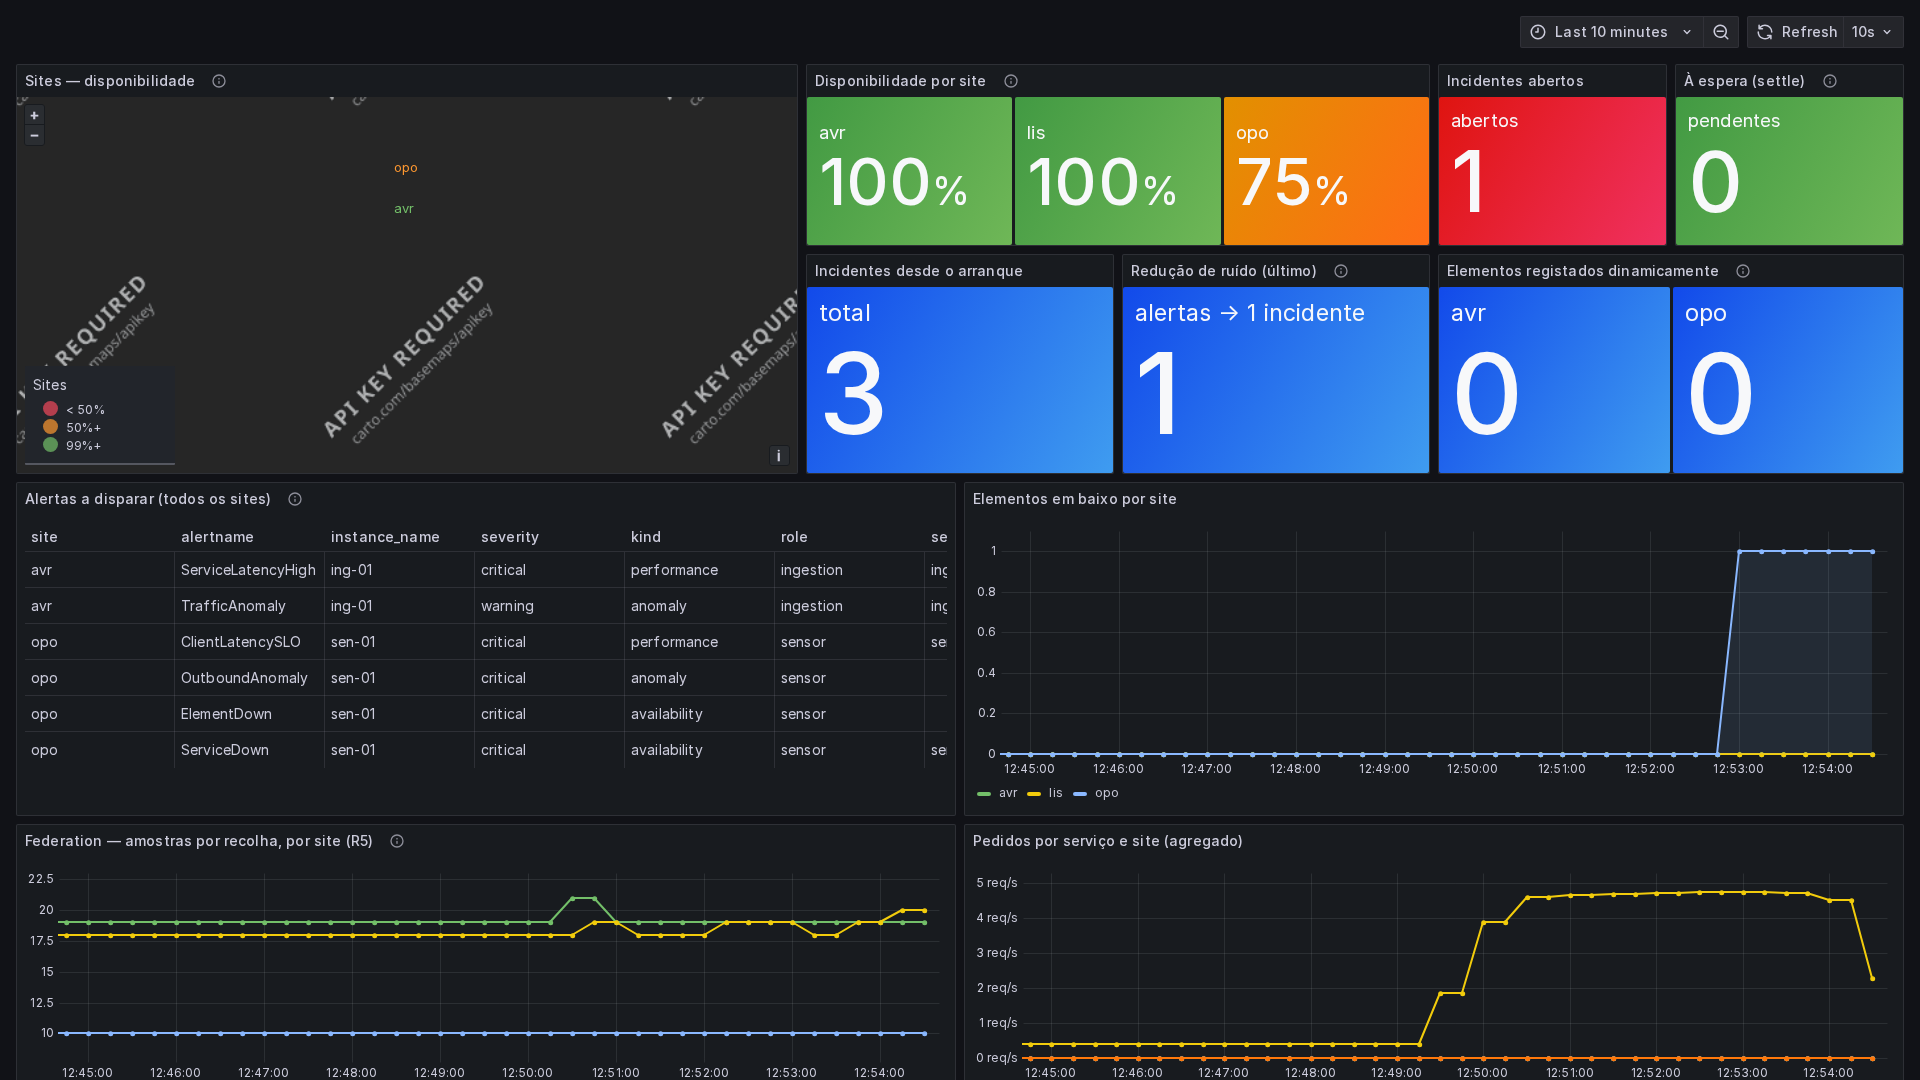
\includegraphics[width=\textwidth]{grafana-soc-t2.png}
  \caption{SOC dashboard during the T2 PoC (live, T490, 22/11, from 2~min before the
    stimulus): \texttt{opo} drops to 75\% (1 of 4 elements down) once \texttt{sen-01} is
    FROZEN (\texttt{incus pause}, 22:12:40), with one open incident and three firing alerts on
    \texttt{sen-01}: \texttt{OutboundAnomaly} (the botnet indicator), \texttt{ElementDown} and
    \texttt{ServiceDown} (consequences of the quarantine itself).}
  \label{fig:soc-t2}
\end{figure}

\subsubsection{Post-mortem}

\paragraph{What the validation caught.} Three of the five rules for this threat were valid
XML but \textbf{would never fire} in the lab. The \texttt{logger} in the PoC lacked the
\texttt{sshd} tag, so the sshd decoder never saw the line. The listening-ports command had a
different alias from the only one rule~533 of the ruleset recognises. And the FIM for
persistence directories was only configured on the \texttt{avr} site, which has no sensors.
None of these defects produces an error: the SIEM starts, the dashboard shows green and the
threat passes.

\paragraph{Quarantine requires the indicator.} Rule~110210 only quarantines a sensor if the
incident carries the \texttt{OutboundAnomaly}. A sensor that is a root cause for another
reason---for example, the \texttt{ClientLatencySLO} of a legitimate sensor during T1 if the
correlator's window fails---is the \textbf{victim}, not a bot: it triggers rule~110211,
without response (negative case in \texttt{cases.json}).

\paragraph{Limitations.} Slow beaconing with jitter evades the traffic anomaly; against this,
rule~110900 joins two weak signals. The emulated brute force uses a fictitious IP
(\texttt{10.10.99.66}), so per-origin response is not exercised here (it is in T1). And a C2
using a common protocol (HTTPS on~443) would not open a new port.


\subsection{Threat 3 --- Junk E-mail from the Infrastructure (Availability / Confidentiality)}
\label{sec:t3}

\subsubsection{Description}

Junk e-mail has two sides. One is volume: an MTA used as a relay, or flooded, wastes queue,
CPU and domain reputation, which affects \textbf{availability}. The other is social: the
content is a social-engineering vector (phishing), which affects \textbf{confidentiality}.
Here the attacker is a compromised internal element (the T2~bot), which
(1)~sends spam to the domain's own mailboxes and
(2)~attempts to use \texttt{mail-01} as an open relay.

\subsubsection{Relevance}

An open relay puts the entire domain on blacklists within hours: the damage escapes the lab
and reaches third parties. It is also the botnet's second ``impact,'' and therefore where the
meta-correlation closes the ``one botnet, two impacts'' story.

\subsubsection{Exploitation / PoC}

\begin{sloppypar}
The MTA is configured with relay only for \texttt{mynetworks} with
explicit \texttt{reject\_unauth\_destination} (the default
\texttt{defer\_unauth\_destination} responds~450, and ruleset
rule~3301 looks for~554); per-client \texttt{anvil}; and \textbf{no mail
leaves the lab} (\texttt{default\_transport = error}). The ``bot'' is a
plain-bash SMTP client that runs on a sensor without installing anything.
It sends $N$ messages with the \textbf{GTUBE} (SpamAssassin's standard
test string) and $M$ relay attempts to \texttt{external.example}.
\end{sloppypar}

\subsubsection{Metrics}

\begin{table}[H]
  \centering
  \caption{T3 detection signals.}
  \begin{tabular}{@{}p{3cm}p{4.5cm}l@{}}
    \toprule
    \textbf{Signal} & \textbf{Source} & \textbf{Rule} \\
    \midrule
    Verdict and score per msg & \texttt{spamd: result: Y 1000 - GTUBE} in \texttt{mail.log} &
      3501 $\to$ 110301 $\to$ \textbf{110304} \\
    Spam volume & 10 marked messages in 2\,min &
      \textbf{110300} \\
    Relay refused per origin & \texttt{554 5.7.1 Relay access denied} $\times 5$ &
      3301 $\to$ \textbf{110302} \\
    Bad reputation origin & CDB \texttt{ssle-reputation} &
      \textbf{110310} \\
    MTA queue & \texttt{postfix\_queue\_messages} &
      Prometheus \\
    Relay from root-cause sensor & Cross-agent correlation &
      \textbf{110900} \\
    \bottomrule
  \end{tabular}
\end{table}

\subsubsection{Detection and Response}

\paragraph{Docker validation} (09/11/2026):

\begin{table}[H]
  \centering
  \caption{T3 Docker validation results.}
  \begin{tabular}{@{}p{4cm}lp{6cm}@{}}
    \toprule
    \textbf{Step} & \textbf{Client sees} & \textbf{SIEM} \\
    \midrule
    1 GTUBE & \texttt{250} &
      \textbf{110304}, score 1002 \\
    10 more GTUBE & \texttt{250$\times$10} &
      \textbf{110300} (wave) \\
    5 relays (client outside \texttt{mynetworks}) & \texttt{554$\times$5} &
      \textbf{110302} $\to$ \texttt{firewall-drop} (alert 651); auto-unblock at 600\,s (652) \\
    Incident ``\texttt{sen-01} is root cause'' + 5 relays from \texttt{sen-01} & \texttt{554} &
      \textbf{110900} (level~14) from 110210 on agent \texttt{obs} \\
    \bottomrule
  \end{tabular}
\end{table}

\paragraph{PoC on the T490 fleet} (14/11/2026, \texttt{mail-01} on \texttt{site-lis}, bots on \texttt{site-opo}):

\begin{table}[H]
  \centering
  \caption{T3 T490 PoC results.}
  \begin{tabular}{@{}p{5.5cm}p{8.5cm}@{}}
    \toprule
    \textbf{Step} & \textbf{Result} \\
    \midrule
    11 GTUBE from \texttt{sen-02} $\to$ \texttt{mail-01} &
      \texttt{250$\times$11} $\cdot$ \textbf{110304}$\times$11 (score 1002) $\cdot$ \textbf{110300} (wave $\geq 10$) \\
    5 relays from \texttt{sen-02} $\to$ \texttt{mail-01} &
      \texttt{554$\times$5} $\cdot$ \texttt{firewall-drop} (iptables DROP \texttt{10.10.2.51}) \\
    6 relays from \texttt{sen-01} (\texttt{ssle\_botnet\_host}) $\to$ \texttt{mail-01} &
      \textbf{110900} (level~14) + \texttt{firewall-drop} of \texttt{10.10.2.50} \\
    \bottomrule
  \end{tabular}
\end{table}

Responses in order of proportionality: MTA rate-limit (\texttt{anvil}), temporary origin
block (\texttt{firewall-drop}, 600\,s), reputation (CDB/RBL) and, if the origin is a
compromised sensor, its quarantine (T2). Planned: SPF/DKIM/DMARC against spoofing.

\subsubsection{Post-mortem}

\paragraph{What the validation caught.} Three defects, all silent.
(1)~The \texttt{spamd} decoder looked for a format that \texttt{spamd} does not write, and
the ruleset's root~3500 always won: spam never generated an alert.
(2)~With the GTUBE each message ends at child rule~110304, and a wave counted over~110301
would never fire (it was changed to count by group).
(3)~When meta-correlation fires, its alert replaces the~110302 alert and
\texttt{firewall-drop} did not run: the bot kept sending (\texttt{firewall-drop} was also
attached to~110900).

\paragraph{Limitations.} The GTUBE proves the chain, not the filter's quality. The MTA
accepts first and filters afterwards (after-queue), so the spam is already in the queue when
detected. And an attacker rotating IPs escapes per-origin blocking, leaving reputation and
\texttt{anvil}.


%% ============================================================================
\section{Evaluation}
\label{sec:evaluation}
%% ============================================================================

\subsection{Detection Effectiveness}

\paragraph{T1, staging (3~runs, 56\,min observation, no response: control group).}

\begin{table}[H]
  \centering
  \caption{T1 staging detection results.}
  \begin{tabular}{@{}lp{8cm}@{}}
    \toprule
    \textbf{Metric} & \textbf{Value} \\
    \midrule
    TP / FP / FN & \textbf{3 / 0 / 0} \\
    MTTD (rule) & $81.7 \pm 2.9$\,s (first signal at 21.7\,s; the rest is \texttt{for: 1m}) \\
    MTTD at SOC & $92.9 \pm 0.1$\,s, correct root cause (\texttt{ing-01}) in all~3 \\
    Mean/std counterproof & Would have detected \textbf{1/3} ($z_{\max} = 3.3$ and 2.8 in runs~2--3) \\
    Server SLO & \textbf{0/3}: server $p_{95} \leq 23.3$\,ms while client felt 242.5\,ms \\
    Client SLO (retroactive) & Would fire at $T_0 + 80$\,s in all~3 \\
    \bottomrule
  \end{tabular}
\end{table}

Two conclusions: (1)~the estimator choice changes the outcome: mean/std ``learns'' the first
attack and becomes blind to subsequent ones. (2)~Measuring only on the server hides the
impact, because the pre-application queue does not appear in the server's histogram. Both
became rules with tests.

\paragraph{T1, T490 (6~runs with SIEM response, against the staging control group):}
see Table~\ref{tab:t1-results}.

\paragraph{T2 (beaconing).} The \texttt{OutboundAnomaly} test yields $z \approx 6.4$ in the
second minute of beaconing on the attacked sensor, no alert on the neighbouring sensor and
none at rest with $\pm 20\%$ legitimate jitter. On the T490, the full chain
(FIM $\to$ SSH $\to$ \texttt{OutboundAnomaly} $\to$ correlator $\to$ quarantine) closes in
${\sim}140$\,s.

\subsection{Correlation}

\begin{table}[H]
  \centering
  \caption{Root-cause correlation results.}
  \label{tab:correlation}
  \begin{tabular}{@{}p{4.5cm}ccp{4.5cm}@{}}
    \toprule
    \textbf{Scenario} & \textbf{Raw alerts} & \textbf{Incidents} & \textbf{Root cause} \\
    \midrule
    Demo: \texttt{sto-01} stopped (live, staging) &
      2 & \textbf{1} & \texttt{sto-01} (not \texttt{ing-01}) \\
    T1: load on \texttt{ing-01} (live, 3$\times$ staging + 10$\times$ T490, 3 of them
      with three origins) &
      1--4/run & 1 & \texttt{ing-01} (13/13) \\
    Client symptom before server (test) &
      2 & 1 & \texttt{ing-01} (with 30\,s window); \texttt{sen-01} without it \\
    Two independent faults (test) &
      2 & 2 & Each its own \\
    \bottomrule
  \end{tabular}
\end{table}

The ten correlator tests use the real inventory graph. On the T490 (15~containers, 3~sites),
correlation was confirmed live: the T1 root cause was identified in all 13~runs, including the
three with origins on three sites, and
T2 produced quarantine of the correct sensor with \texttt{OutboundAnomaly} as the indicator.

\subsection{False Positives over an Attack-Free Window}
\label{sec:fp}

Every alert in the earlier sections answers a stimulus. To measure the opposite, the lab was
left running \textbf{untouched for 10.1~h} after the last PoC (22/11 22:24 to 23/11 08:30 UTC):
15~containers, 14~agents, the sensors sending readings, no stimulus and no operator activity.
Anything that fires in that window is, by definition, a false positive.
\texttt{evaluation/fp-window.sh} counts it from the sources: firing episodes of \texttt{ALERTS}
on the three site Prometheus servers and on the global one, incidents opened by the correlator,
Wazuh alerts (project rules at level~$\geq 7$ and any rule at level~$\geq 10$) and active
responses executed on every agent that has one. All 30~scrape targets stayed up for the whole
window (13\,s of data gaps in total).

\begin{table}[H]
  \centering
  \caption{False positives over a 10.1-hour attack-free window (T490, 22--23/11).}
  \label{tab:fp}
  \begin{tabular}{@{}lccl@{}}
    \toprule
    \textbf{Source} & \textbf{Events} & \textbf{Per hour} & \textbf{Closest approach to the threshold} \\
    \midrule
    Prometheus (4 servers) & 0 & 0 & \texttt{TrafficAnomaly} $z = 0.09$, \texttt{OutboundAnomaly} $z = 0.89$ (of 3) \\
    & & & server p95 5\,ms, client p95 39\,ms (of 100\,ms); errors 0\,\% \\
    Correlator incidents & 0 & 0 & --- \\
    Wazuh alerts & 0 & 0 & no alert at any level $\geq 3$; no events dropped \\
    Active responses & 0 & 0 & --- \\
    \bottomrule
  \end{tabular}
\end{table}

The same idle lab was \textbf{not} silent before defect~19 was fixed. A duplicate
\texttt{netstat} alias in the agent configuration made rule~533 report a ``changed'' listening
port on every check, and rule~110202 (level~10, the T2 indicator ``new listening port'')
fired about 20~times per hour on each sensor: 40~times on each of \texttt{sen-01} and
\texttt{sen-02} in 1.9~h on 19/11, and 14~times each in the 45~minutes before the fix on
22/11. That is roughly 40~level-10 false positives per hour with no attack at all. No sensor
was quarantined, because quarantine also needs the correlator's \texttt{OutboundAnomaly}
incident, but the SOC queue was flooded with exactly the alert that should announce a botnet.
After the fix (\texttt{install-agent.sh} now removes the default \texttt{netstat} block, and
\texttt{it-agents.sh} checks that it is gone), the same rule stayed silent for the whole 10.1~h.

\paragraph{What this does and does not show.} Zero events in 10.1~h bounds the rate at
roughly ${\leq}\,0.3$ false positives per hour (95\,\% upper bound, rule of three: $3/10.1$).
The bound holds for \emph{this} baseline only. Idle lab traffic is very regular (about
0.44~req/s on \texttt{ing-01}), so the IQR floor of the robust $z$ dominates and the score barely
moves. Real traffic, with daily cycles, deployments and legitimate bursts, will come closer to
the thresholds. The window shows that the rules do not fire on normal operation of the system
as built, and that the one rule that did was a defect, not noise to be tuned away.

\subsection{SIEM and Response Validation}

\begin{table}[H]
  \centering
  \caption{SIEM validation results.}
  \begin{tabular}{@{}p{3.5cm}p{5cm}p{4cm}@{}}
    \toprule
    \textbf{Level} & \textbf{What it exercises} & \textbf{Result} \\
    \midrule
    Load on \texttt{analysisd} 4.14.10 &
      Rule syntax, decoders, lists and responses & 0~errors, 0~warnings \\
    25 assertion cases &
      Each rule 1100xx--1109xx, with negative cases & 25/25 \\
    Response unit tests &
      Quarantine (fake \texttt{incus}) and rate-limit (real nft in namespace) & 19/19 \\
    Integration with real agents &
      5~agents + real MTA, stimulus to response & 34/34 \\
    \bottomrule
  \end{tabular}
\end{table}

Along the way, \textbf{19~defects} appeared: 2~fatal at load, 7~caught by assertion cases,
8~only with real agents and 2~only in the live lab. Of these~19, 16~were silent: the SIEM
started, the dashboard showed green and the threat passed. The last two were found by tests
shaped like reality rather than like the rule: a T1 with three origins showed that the
``all origins'' response of 110101/110110 had \textbf{never engaged} since the first run
(Section~\ref{sec:t1}), and the attack-free window showed rule~110202 firing with no port
change at all (Section~\ref{sec:fp}). This is the strongest process result of this work: in a
detection system, a test that only checks that the configuration loads tests nothing.

\subsection{Federation Bandwidth and Scale}

\paragraph{Bandwidth (measured without the lab).} A real Prometheus~2.53.5 with the project's
site rules, scraping $N$~elements over real exporters. Compares what the global pulls with
the project's \texttt{match[]} against what a central Prometheus \textbf{without hierarchy}
would pull (all time series):

\begin{table}[H]
  \centering
  \caption{Federation bandwidth savings.}
  \begin{tabular}{@{}rp{3.5cm}p{3.5cm}r@{}}
    \toprule
    \textbf{$N$ elements} & \textbf{Series: agg.\ / all} & \textbf{Bytes/req (gzip): agg.\ / all} &
      \textbf{Savings} \\
    \midrule
    10 & 25 / 8\,225 & 443\,B / 64.8\,kB & 99.3\,\% \\
    25 & 55 / 20\,555 & 689\,B / 150.7\,kB & 99.5\,\% \\
    50 & 105 / 41\,105 & 1.0\,kB / 300.8\,kB & 99.7\,\% \\
    \bottomrule
  \end{tabular}
\end{table}

The federated series are $2N + 5$: 5~site aggregates (constant) plus the \texttt{up} of each
target, retained because the global root-cause analysis needs to know \textbf{which} element
is down. The global federates every 30\,s (2~requests/min), so a site of 50~elements costs
\textbf{2.1\,kB/min} between sites, against 0.6\,MB/min without hierarchy. Savings grow with $N$, because each
element adds 2~series on one side and ${\sim}820$ on the other.

\paragraph{Lab scale (T490, 14/11, 15~containers, 12~elements across 3~sites):}

\begin{table}[H]
  \centering
  \caption{Prometheus resource usage on the T490.}
  \begin{tabular}{@{}lrrrrr@{}}
    \toprule
    \textbf{Instance} & \textbf{Targets} & \textbf{Series} & \textbf{Ingestion} &
      \textbf{RSS} & \textbf{CPU} \\
    \midrule
    site-avr (5 elements) & 9 & 7\,577 & 502\,samples/s & 26.5\,MiB & 1.6\,\% \\
    site-opo (4 elements) & 8 & 6\,300 & 417\,samples/s & 26.8\,MiB & 1.4\,\% \\
    site-lis (3 elements)  & 5 & 4\,750 & 315\,samples/s & 25.9\,MiB & 1.4\,\% \\
    obs (global, 3 federates) & 8 & 4\,428 & 147\,samples/s & 26.0\,MiB & 0.7\,\% \\
    \bottomrule
  \end{tabular}
\end{table}

The heaviest scrape is \texttt{node\_exporter} (265--334\,ms, ${\sim}1\,331$ samples); the
Flask service scrape takes $< 5$\,ms (14--30~samples). Federation costs 1--3\,ms per site
(10--19~series, 1.1\,kB gzip). Recording-rule evaluation takes 8--11\,ms per cycle on the
sites and $< 1$\,ms on the global.

The heaviest component is Wazuh (3.3\,GiB); each site Prometheus occupies
${\sim}480$--$497$\,MiB (includes the \texttt{node\_exporter}, OS and container services).
The total for 15~containers is \textbf{${\sim}8.3$\,GiB} on the host's 24\,GiB RAM
(16\,GiB free). At 50~elements per site (150~total), the series count and ingestion grow
linearly (${\sim}1\,350$~series/element), but the Prometheus RSS grows little: in staging,
50~synthetic elements (with the same real exporters) produced 41\,105~series and the
Prometheus did not exceed 35\,MiB RSS---the dominant cost is disk (TSDB) and network.

\subsection{Threats to Validity}

\begin{itemize}
  \item T1 was measured in staging (control group) and on the T490 (with response), with the
    same software and the same stimulus script, but \textbf{not the same delivered load}:
    ${\sim}160$~requests/s in staging against ${\sim}21$~requests/s on the T490, where the
    service is slower and the per-origin limiter binds within seconds. The
    detection rule is relative (robust $z$ against each instance's own baseline) and both
    loads are far above its threshold ($z_{\max} \approx 320$ and $\approx 42$), so MTTD is
    comparable; absolute latencies and the server-SLO outcome are not.
  \item The SIEM validation ran in Docker, without \texttt{systemd} or Incus. The scripts are
    from the deploy, but the installation and timing in the lab differ.
  \item The PoCs are benign emulations: SSH brute force is logged with \texttt{logger} (there
    is no \texttt{sshd}), and the spam is the GTUBE. They prove the detection and response
    chain, not the detection of a real adversary.
\end{itemize}


%% ============================================================================
\section{Conclusions}
\label{sec:conclusions}
%% ============================================================================

\subsection{Summary of Results}

This work shows that a detection system for a distributed infrastructure can be built and
\textbf{proved as code}, from a single source of truth. From the inventory come the network,
fleet, monitoring targets, dependency graph and SIEM configuration. The main results are
four.

First, \textbf{robust} anomaly detection (median/IQR) detected all 13~T1 runs (MTTD ${\sim}80$\,s),
where mean/std would have missed seven, and raised no alert over a 10-hour attack-free window. The SIEM response
(rule~110100 $\to$ \texttt{ssle-ratelimit} nft) activates in ${\sim}6$\,s, more than ten
times faster than metric-based detection, and drops 597--1\,098 packets per run (runs 7--9) without
affecting the legitimate sensors.

Second, graph-based correlation reduced $N$ alerts to \textbf{one} incident with the correct
root cause, even with the cause on one site and the symptoms on another.

Third, all three threats have detection \textbf{and} proportional, reversible response,
proved from stimulus to action on the correct agent: quarantine in ${\sim}140$\,s (T2) and
\texttt{firewall-drop} in $< 10$\,s (T3).

Fourth, meta-correlation links the threats: a sensor that is a root cause of anomaly
\textbf{and} the origin of an impact is treated as a bot (rule~110900, level~14).

The methodological lesson carries the most weight: \textbf{``loads without errors'' does not
mean ``detects.''} Of the 19~defects found in the SIEM, 16~were valid configuration that
never fired, misfired or never acted, and only appeared with tests that assert ``this event
must produce this rule,'' with real agents, and with live runs shaped like the real attack.

\subsection{Limitations}

\begin{itemize}
  \item \textbf{Single host.} The three sites share the same hypervisor. Inter-site latencies
    are those of a local bridge, and a host failure takes everything, including the SOC. The
    architecture does not depend on this (sites communicate only by IP), but the measurements
    do.
  \item \textbf{The baseline can be trained.} The robust z-score resists an attack occupying
    less than 25\,\% of the window (the IQR's breakdown point). A patient attacker raising
    the load slowly moves the median with it. The absolute rules (client SLO) are the safety
    net, but only for what the client feels.
  \item \textbf{Correlation costs time.} The settle window (30\,s) prevents blaming the wrong
    sensor, but adds up to 30\,s to SOC MTTD. This is a conscious trade-off between speed
    and certainty.
  \item \textbf{Detection is reactive.} Wazuh sees the event after it happens. The MTA
    accepts spam before filtering it (after-queue), and the T1 rate-limit activates after
    detection, not proactively.
  \item \textbf{Automatic responses can cause harm.} A false positive of
    \texttt{OutboundAnomaly} pauses a legitimate sensor for 10\,min. Hence quarantine only
    acts on sensors, only with the botnet indicator and always with \texttt{timeout}. The
    \texttt{responder} has power over all sites: the restricted certificate removes the core,
    but not the sites.
  \item \textbf{The attacker adapts.} A slow C2 over~443 with jitter evades the connection
    anomaly; a bot rotating IPs evades per-origin blocking; real spam with an untrained Bayes
    has false negatives (the GTUBE proves the chain, not the filter quality).
  \item \textbf{The SIEM has its own semantics.} Composite-rule state is per-agent and
    \texttt{ignore} is per-rule. Both are handled today, but any new rule that ignores them
    recreates silent holes. The antidote is testing, not review.
  \item \textbf{Validation outside the lab.} The SIEM integration ran first in Docker
    (without \texttt{systemd} or Incus) and then on the T490 (15~containers, 14~agents). The
    three PoCs and responses are validated in both environments, but the lab remains on a
    single physical host.
\end{itemize}

\subsection{Future Work}

\begin{itemize}
  \item \textbf{Attack tolerance (bridge to Project~2):} a second ingestion replica,
    discovered by the site registry, so that the T1 response can be ``scale out'' rather than
    just ``limit,'' and aggregate admission control (a global limit or fast 503s) for attacks
    spread below the per-origin threshold (Table~\ref{tab:t1-ddos}).
  \item \textbf{Proactive prevention:} per-origin rate-limit always active at the entry of
    exposed services and SPF/DKIM/DMARC on the MTA.
  \item \textbf{Automatic reimaging} from reference snapshots as a T2 response, after
    forensics.
  \item \textbf{Scale beyond the lab:} with 50~elements per site, federation saves
    $> 99$\,\% of bandwidth (2.1\,kB/min per site); the site Prometheus uses $< 27$\,MiB RSS
    and $< 2$\,\% CPU. Validation with 150+ real elements on distinct hardware (multiple
    hosts, WAN latencies) remains to be done.
\end{itemize}


\subsection{AI Usage Disclosure}

This project made extensive use of generative AI. The large majority of the AI-assisted work
was done with \textbf{Claude Opus~4.6} (Anthropic), used as a coding and writing assistant.
It was used for:

\begin{itemize}
  \item \textbf{Automation:} writing the deployment and test automation---Incus container
    provisioning, inventory-driven generation of networks, Prometheus targets, Wazuh agent
    enrolment and configuration, and the scripts that run the PoCs and collect evidence.
  \item \textbf{Architecture decisions:} discussing the design of the Incus lab and reaching
    decisions with the model's help---one Incus project and network per site, hierarchical
    Prometheus federation, the dependency graph for root-cause correlation, the TTL-based site
    registry and the restricted certificate for the responder. The final choices and their
    validation on the lab were the author's responsibility.
  \item \textbf{Monitoring and SIEM configuration:} Grafana dashboards, Prometheus rules, Wazuh
    rules and the correlator, including tests for edge cases such as per-agent composite-rule
    state and the \texttt{ignore} semantics.
  \item \textbf{Writing the report in \LaTeX:} structuring sections, phrasing technical
    descriptions, tables and formatting, and keeping the repository documentation in a single
    language (English).
\end{itemize}

The author reviewed the AI-generated output and is responsible for it. The measurements and
results reported here come from real executions on the lab (T490, 15~Incus containers) and
in the Docker-based integration environment, not from the model.

%% ============================================================================
\begin{thebibliography}{15}
\bibitem{iso7498}
  ISO/IEC~7498-4:1989,
  \emph{Information processing systems---OSI Basic Reference Model---Part~4: Management
  framework}.

\bibitem{brazil2018}
  B.~Brazil,
  \emph{Prometheus: Up \& Running},
  O'Reilly, 2018.

\bibitem{sre2016}
  B.~Beyer, C.~Jones, J.~Petoff, N.\,R.~Murphy (eds.),
  \emph{Site Reliability Engineering},
  O'Reilly, 2016.

\bibitem{iglewicz1993}
  B.~Iglewicz, D.\,C.~Hoaglin,
  \emph{How to Detect and Handle Outliers},
  ASQC Quality Press, 1993.

\bibitem{steinder2004}
  M.~Steinder, A.\,S.~Sethi,
  ``A survey of fault localization techniques in computer networks,''
  \emph{Science of Computer Programming}, 53(2):165--194, 2004.

\bibitem{kliger1995}
  S.~Kliger, S.~Yemini, Y.~Yemini, D.~Ohsie, S.~Stolfo,
  ``A coding approach to event correlation,''
  in \emph{Proc.\ IFIP/IEEE Int.\ Symp.\ on Integrated Network Management (ISINM)}, 1995.

\bibitem{wazuh}
  Wazuh,
  \emph{Wazuh documentation}, version~4.14,
  \url{https://documentation.wazuh.com/4.14/}.

\bibitem{kordy2014}
  B.~Kordy, S.~Mauw, S.~Radomirovi\'c, P.~Schweitzer,
  ``Attack--defence trees,''
  \emph{Journal of Logic and Computation}, 24(1):55--87, 2014.

\bibitem{mitre2024}
  MITRE Corporation,
  \emph{MITRE ATT\&CK\textregistered\ Enterprise Matrix}, version~15,
  2024.
  \url{https://attack.mitre.org/}.

\bibitem{kolias2017}
  C.~Kolias, G.~Kambourakis, A.~Stavrou, J.~Voas,
  ``DDoS in the IoT: Mirai and other botnets,''
  \emph{Computer}, 50(7):80--84, IEEE, 2017.

\bibitem{antonakakis2017}
  M.~Antonakakis \emph{et~al.},
  ``Understanding the Mirai botnet,''
  in \emph{Proc.\ 26th USENIX Security Symp.}, pp.~1093--1110, 2017.

\bibitem{bertino2017}
  E.~Bertino, N.~Islam,
  ``Botnets and Internet of Things security,''
  \emph{Computer}, 50(2):76--79, IEEE, 2017.

\bibitem{scarfone2007}
  K.~Scarfone, P.~Mell,
  ``Guide to Intrusion Detection and Prevention Systems (IDPS),''
  NIST SP~800-94, 2007.

\bibitem{prometheus2024}
  Prometheus Authors,
  \emph{Prometheus documentation: Federation},
  2024.
  \url{https://prometheus.io/docs/prometheus/latest/federation/}.

\bibitem{chuvakin2012}
  A.~Chuvakin, K.~Schmidt, C.~Phillips,
  \emph{Logging and Log Management: The Authoritative Guide to Dealing with Syslog, Audit Logs, Events, Alerts and Other IT Noise},
  Syngress, 2012.
\end{thebibliography}

\end{document}
